\documentclass[twoside]{book}

% Packages required by doxygen
\usepackage{calc}
\usepackage{doxygen}
\usepackage{graphicx}
\usepackage[utf8]{inputenc}
\usepackage{makeidx}
\usepackage{multicol}
\usepackage{multirow}
\usepackage{textcomp}
\usepackage[table]{xcolor}

% NLS support packages
\usepackage[ngerman]{babel}

% Font selection
\usepackage[T1]{fontenc}
\usepackage{mathptmx}
\usepackage[scaled=.90]{helvet}
\usepackage{courier}
\usepackage{amssymb}
\usepackage{sectsty}
\renewcommand{\familydefault}{\sfdefault}
\allsectionsfont{%
  \fontseries{bc}\selectfont%
  \color{darkgray}%
}
\renewcommand{\DoxyLabelFont}{%
  \fontseries{bc}\selectfont%
  \color{darkgray}%
}

% Page & text layout
\usepackage{geometry}
\geometry{%
  a4paper,%
  top=2.5cm,%
  bottom=2.5cm,%
  left=2.5cm,%
  right=2.5cm%
}
\tolerance=750
\hfuzz=15pt
\hbadness=750
\setlength{\emergencystretch}{15pt}
\setlength{\parindent}{0cm}
\setlength{\parskip}{0.2cm}
\makeatletter
\renewcommand{\paragraph}{%
  \@startsection{paragraph}{4}{0ex}{-1.0ex}{1.0ex}{%
    \normalfont\normalsize\bfseries\SS@parafont%
  }%
}
\renewcommand{\subparagraph}{%
  \@startsection{subparagraph}{5}{0ex}{-1.0ex}{1.0ex}{%
    \normalfont\normalsize\bfseries\SS@subparafont%
  }%
}
\makeatother

% Headers & footers
\usepackage{fancyhdr}
\pagestyle{fancyplain}
\fancyhead[LE]{\fancyplain{}{\bfseries\thepage}}
\fancyhead[CE]{\fancyplain{}{}}
\fancyhead[RE]{\fancyplain{}{\bfseries\leftmark}}
\fancyhead[LO]{\fancyplain{}{\bfseries\rightmark}}
\fancyhead[CO]{\fancyplain{}{}}
\fancyhead[RO]{\fancyplain{}{\bfseries\thepage}}
\fancyfoot[LE]{\fancyplain{}{}}
\fancyfoot[CE]{\fancyplain{}{}}
\fancyfoot[RE]{\fancyplain{}{\bfseries\scriptsize Erzeugt am Die Jun 18 2013 18:27:13 für Service-Interface für ein Formula Student Fahrzeug von Doxygen }}
\fancyfoot[LO]{\fancyplain{}{\bfseries\scriptsize Erzeugt am Die Jun 18 2013 18:27:13 für Service-Interface für ein Formula Student Fahrzeug von Doxygen }}
\fancyfoot[CO]{\fancyplain{}{}}
\fancyfoot[RO]{\fancyplain{}{}}
\renewcommand{\footrulewidth}{0.4pt}
\renewcommand{\chaptermark}[1]{%
  \markboth{#1}{}%
}
\renewcommand{\sectionmark}[1]{%
  \markright{\thesection\ #1}%
}

% Indices & bibliography
\usepackage{natbib}
\usepackage[titles]{tocloft}
\setcounter{tocdepth}{3}
\setcounter{secnumdepth}{5}
\makeindex

% Hyperlinks (required, but should be loaded last)
\usepackage{ifpdf}
\ifpdf
  \usepackage[pdftex,pagebackref=true]{hyperref}
\else
  \usepackage[ps2pdf,pagebackref=true]{hyperref}
\fi
\hypersetup{%
  colorlinks=true,%
  linkcolor=blue,%
  citecolor=blue,%
  unicode%
}

% Custom commands
\newcommand{\clearemptydoublepage}{%
  \newpage{\pagestyle{empty}\cleardoublepage}%
}


%===== C O N T E N T S =====

\begin{document}

% Titlepage & ToC
\hypersetup{pageanchor=false}
\pagenumbering{roman}
\begin{titlepage}
\vspace*{7cm}
\begin{center}%
{\Large Service-\/\-Interface für ein Formula Student Fahrzeug }\\
\vspace*{1cm}
{\large Erzeugt von Doxygen 1.8.4}\\
\vspace*{0.5cm}
{\small Die Jun 18 2013 18:27:13}\\
\end{center}
\end{titlepage}
\clearemptydoublepage
\tableofcontents
\clearemptydoublepage
\pagenumbering{arabic}
\hypersetup{pageanchor=true}

%--- Begin generated contents ---
\chapter{Hierarchie-\/\-Verzeichnis}
\section{Class Hierarchy}
This inheritance list is sorted roughly, but not completely, alphabetically\-:\begin{DoxyCompactList}
\item \contentsline{section}{Data}{\pageref{classData}}{}
\item \contentsline{section}{Decoder}{\pageref{classDecoder}}{}
\item \contentsline{section}{Encoder}{\pageref{classEncoder}}{}
\item exception\begin{DoxyCompactList}
\item \contentsline{section}{Socket\-Exception}{\pageref{classSocketException}}{}
\end{DoxyCompactList}
\item \contentsline{section}{Location}{\pageref{classLocation}}{}
\item \contentsline{section}{Receiver}{\pageref{classReceiver}}{}
\item \contentsline{section}{Sender}{\pageref{classSender}}{}
\item \contentsline{section}{Socket}{\pageref{classSocket}}{}
\begin{DoxyCompactList}
\item \contentsline{section}{Communicating\-Socket}{\pageref{classCommunicatingSocket}}{}
\begin{DoxyCompactList}
\item \contentsline{section}{T\-C\-P\-Socket}{\pageref{classTCPSocket}}{}
\item \contentsline{section}{U\-D\-P\-Socket}{\pageref{classUDPSocket}}{}
\end{DoxyCompactList}
\item \contentsline{section}{T\-C\-P\-Server\-Socket}{\pageref{classTCPServerSocket}}{}
\end{DoxyCompactList}
\item \contentsline{section}{T\-\_\-nuex}{\pageref{structT__nuex}}{}
\end{DoxyCompactList}

\chapter{Klassen-\/\-Verzeichnis}
\section{Auflistung der Klassen}
Hier folgt die Aufzählung aller Klassen, Strukturen, Varianten und Schnittstellen mit einer Kurzbeschreibung\-:\begin{DoxyCompactList}
\item\contentsline{section}{\hyperlink{classCommunicatingSocket}{Communicating\-Socket} }{\pageref{classCommunicatingSocket}}{}
\item\contentsline{section}{\hyperlink{classData}{Data} }{\pageref{classData}}{}
\item\contentsline{section}{\hyperlink{classDatatypeDaemon}{Datatype\-Daemon} \\*Klasse zum Aufbereiten der Daten }{\pageref{classDatatypeDaemon}}{}
\item\contentsline{section}{\hyperlink{classdbData}{db\-Data} \\*Klasse zum Auslesen der Zugangsdaten f"ur die Datenbank }{\pageref{classdbData}}{}
\item\contentsline{section}{\hyperlink{classDBPacketInsert}{D\-B\-Packet\-Insert} }{\pageref{classDBPacketInsert}}{}
\item\contentsline{section}{\hyperlink{classDecoder}{Decoder} }{\pageref{classDecoder}}{}
\item\contentsline{section}{\hyperlink{classEncoder}{Encoder} }{\pageref{classEncoder}}{}
\item\contentsline{section}{\hyperlink{classInsert}{Insert} \\*Klasse zum Aufbauen einer Verbindung zur Datenbank und Einf"ugen von Daten }{\pageref{classInsert}}{}
\item\contentsline{section}{\hyperlink{classLocation}{Location} }{\pageref{classLocation}}{}
\item\contentsline{section}{\hyperlink{classSocket}{Socket} }{\pageref{classSocket}}{}
\item\contentsline{section}{\hyperlink{classSocketException}{Socket\-Exception} }{\pageref{classSocketException}}{}
\item\contentsline{section}{\hyperlink{structT__nuex}{T\-\_\-nuex} }{\pageref{structT__nuex}}{}
\item\contentsline{section}{\hyperlink{classTCPServerSocket}{T\-C\-P\-Server\-Socket} }{\pageref{classTCPServerSocket}}{}
\item\contentsline{section}{\hyperlink{classTCPSocket}{T\-C\-P\-Socket} }{\pageref{classTCPSocket}}{}
\item\contentsline{section}{\hyperlink{classUDPSocket}{U\-D\-P\-Socket} }{\pageref{classUDPSocket}}{}
\end{DoxyCompactList}

\chapter{Klassen-\/\-Dokumentation}
\hypertarget{classCommunicatingSocket}{\section{Communicating\-Socket Klassenreferenz}
\label{classCommunicatingSocket}\index{Communicating\-Socket@{Communicating\-Socket}}
}


{\ttfamily \#include $<$Practical\-Socket.\-h$>$}

Klassendiagramm für Communicating\-Socket\-:\begin{figure}[H]
\begin{center}
\leavevmode
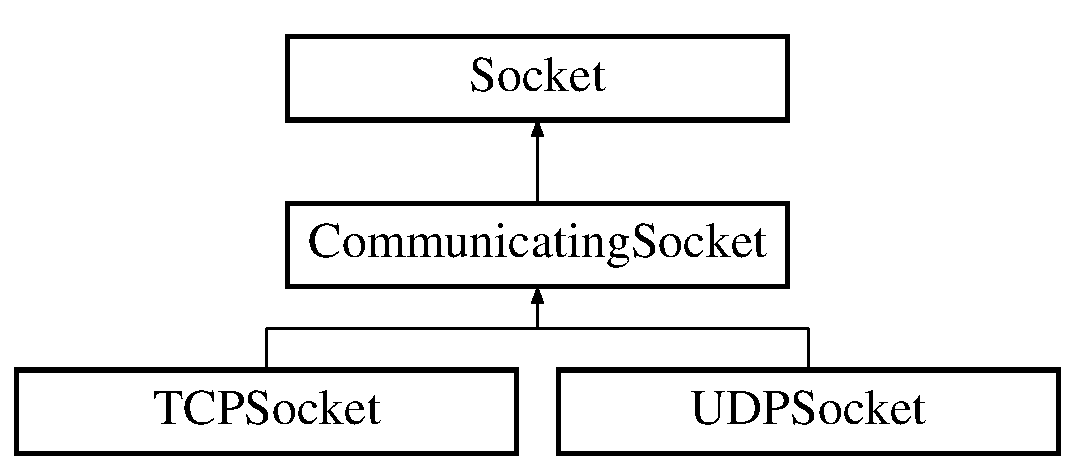
\includegraphics[height=3.000000cm]{classCommunicatingSocket}
\end{center}
\end{figure}
\subsection*{Öffentliche Methoden}
\begin{DoxyCompactItemize}
\item 
void \hyperlink{classCommunicatingSocket_a9192374d9baab8e189860aa8d913683c}{connect} (const string \&foreign\-Address, unsigned short foreign\-Port)  throw (\-Socket\-Exception)
\item 
void \hyperlink{classCommunicatingSocket_aca4e86085c064641e86ae24ea29bbb94}{send} (const void $\ast$buffer, int buffer\-Len)  throw (\-Socket\-Exception)
\item 
int \hyperlink{classCommunicatingSocket_a7cf1fd470c0060171b68df9f68c7bd01}{recv} (void $\ast$buffer, int buffer\-Len)  throw (\-Socket\-Exception)
\item 
string \hyperlink{classCommunicatingSocket_a13f9eca30ef56836cf23c163c848c09e}{get\-Foreign\-Address} ()  throw (\-Socket\-Exception)
\item 
unsigned short \hyperlink{classCommunicatingSocket_a184fbb4775184b87ebd886a5587eb1a3}{get\-Foreign\-Port} ()  throw (\-Socket\-Exception)
\end{DoxyCompactItemize}
\subsection*{Geschützte Methoden}
\begin{DoxyCompactItemize}
\item 
\hypertarget{classCommunicatingSocket_a0017517b8d6e761fde0c40475af3b2ab}{{\bfseries Communicating\-Socket} (int type, int protocol)  throw (\-Socket\-Exception)}\label{classCommunicatingSocket_a0017517b8d6e761fde0c40475af3b2ab}

\item 
\hypertarget{classCommunicatingSocket_a27d758db782b3be7d28741e92cb613d1}{{\bfseries Communicating\-Socket} (int new\-Conn\-S\-D)}\label{classCommunicatingSocket_a27d758db782b3be7d28741e92cb613d1}

\end{DoxyCompactItemize}
\subsection*{Weitere Geerbte Elemente}


\subsection{Ausführliche Beschreibung}
\hyperlink{classSocket}{Socket} der in der Lage ist sich zu verbinden, zu senden und zu empfangen. 

\subsection{Dokumentation der Elementfunktionen}
\hypertarget{classCommunicatingSocket_a9192374d9baab8e189860aa8d913683c}{\index{Communicating\-Socket@{Communicating\-Socket}!connect@{connect}}
\index{connect@{connect}!CommunicatingSocket@{Communicating\-Socket}}
\subsubsection[{connect}]{\setlength{\rightskip}{0pt plus 5cm}void Communicating\-Socket\-::connect (
\begin{DoxyParamCaption}
\item[{const string \&}]{foreign\-Address, }
\item[{unsigned short}]{foreign\-Port}
\end{DoxyParamCaption}
) throw  {\bf Socket\-Exception}) }}\label{classCommunicatingSocket_a9192374d9baab8e189860aa8d913683c}
Baut eine Verbindung "uber Sockets zu einem bestimmten Teilnehmer. 
\begin{DoxyParams}{Parameter}
{\em foreign\-Address} & Adresse des Teilnehmers (I\-P Adresse oder Name). \\
\hline
{\em foreign\-Port} & Portnummer des Teilnehmers. \\
\hline
\end{DoxyParams}

\begin{DoxyExceptions}{Ausnahmebehandlung}
{\em \hyperlink{classSocketException}{Socket\-Exception}} & wird geworfen wenn die Verbindung fehlschl"agt. \\
\hline
\end{DoxyExceptions}
\hypertarget{classCommunicatingSocket_a13f9eca30ef56836cf23c163c848c09e}{\index{Communicating\-Socket@{Communicating\-Socket}!get\-Foreign\-Address@{get\-Foreign\-Address}}
\index{get\-Foreign\-Address@{get\-Foreign\-Address}!CommunicatingSocket@{Communicating\-Socket}}
\subsubsection[{get\-Foreign\-Address}]{\setlength{\rightskip}{0pt plus 5cm}string Communicating\-Socket\-::get\-Foreign\-Address (
\begin{DoxyParamCaption}
{}
\end{DoxyParamCaption}
) throw  {\bf Socket\-Exception}) }}\label{classCommunicatingSocket_a13f9eca30ef56836cf23c163c848c09e}
Holt die Zieladresse. \begin{DoxyReturn}{Rückgabe}
Zieladresse. 
\end{DoxyReturn}

\begin{DoxyExceptions}{Ausnahmebehandlung}
{\em \hyperlink{classSocketException}{Socket\-Exception}} & wird geworfen falls das Holen fehlschl"agt. \\
\hline
\end{DoxyExceptions}
\hypertarget{classCommunicatingSocket_a184fbb4775184b87ebd886a5587eb1a3}{\index{Communicating\-Socket@{Communicating\-Socket}!get\-Foreign\-Port@{get\-Foreign\-Port}}
\index{get\-Foreign\-Port@{get\-Foreign\-Port}!CommunicatingSocket@{Communicating\-Socket}}
\subsubsection[{get\-Foreign\-Port}]{\setlength{\rightskip}{0pt plus 5cm}unsigned short Communicating\-Socket\-::get\-Foreign\-Port (
\begin{DoxyParamCaption}
{}
\end{DoxyParamCaption}
) throw  {\bf Socket\-Exception}) }}\label{classCommunicatingSocket_a184fbb4775184b87ebd886a5587eb1a3}
Holt den Zielport. Call \hyperlink{classCommunicatingSocket_a9192374d9baab8e189860aa8d913683c}{connect()} before calling \hyperlink{classCommunicatingSocket_a7cf1fd470c0060171b68df9f68c7bd01}{recv()} \begin{DoxyReturn}{Rückgabe}
Zielportnummer. 
\end{DoxyReturn}

\begin{DoxyExceptions}{Ausnahmebehandlung}
{\em \hyperlink{classSocketException}{Socket\-Exception}} & wird geworfen falls das Holen fehlschl"agt. \\
\hline
\end{DoxyExceptions}
\hypertarget{classCommunicatingSocket_a7cf1fd470c0060171b68df9f68c7bd01}{\index{Communicating\-Socket@{Communicating\-Socket}!recv@{recv}}
\index{recv@{recv}!CommunicatingSocket@{Communicating\-Socket}}
\subsubsection[{recv}]{\setlength{\rightskip}{0pt plus 5cm}int Communicating\-Socket\-::recv (
\begin{DoxyParamCaption}
\item[{void $\ast$}]{buffer, }
\item[{int}]{buffer\-Len}
\end{DoxyParamCaption}
) throw  {\bf Socket\-Exception}) }}\label{classCommunicatingSocket_a7cf1fd470c0060171b68df9f68c7bd01}
Ließt eine Nachricht in den "ubergebenen Buffer ein. \hyperlink{classCommunicatingSocket_a9192374d9baab8e189860aa8d913683c}{connect()} muss vorher aufgerufen werden. 
\begin{DoxyParams}{Parameter}
{\em buffer} & Speicher in den die Nachricht geschrieben werden soll. \\
\hline
{\em buffer\-Len} & Maximale Anzahl an Bytes die empfangen werden sollen. \\
\hline
\end{DoxyParams}
\begin{DoxyReturn}{Rückgabe}
Gibt die Anzahl der gelesenen Bytes zur"uck. 0 wenn E\-O\-F und -\/1 im Fehlerfall. 
\end{DoxyReturn}

\begin{DoxyExceptions}{Ausnahmebehandlung}
{\em \hyperlink{classSocketException}{Socket\-Exception}} & wird geworfen falls keine Daten emfpangen werden k"onnen. \\
\hline
\end{DoxyExceptions}
\hypertarget{classCommunicatingSocket_aca4e86085c064641e86ae24ea29bbb94}{\index{Communicating\-Socket@{Communicating\-Socket}!send@{send}}
\index{send@{send}!CommunicatingSocket@{Communicating\-Socket}}
\subsubsection[{send}]{\setlength{\rightskip}{0pt plus 5cm}void Communicating\-Socket\-::send (
\begin{DoxyParamCaption}
\item[{const void $\ast$}]{buffer, }
\item[{int}]{buffer\-Len}
\end{DoxyParamCaption}
) throw  {\bf Socket\-Exception}) }}\label{classCommunicatingSocket_aca4e86085c064641e86ae24ea29bbb94}
Schreibt den "ubergebenen Buffer in den \hyperlink{classSocket}{Socket}. Vor \hyperlink{classCommunicatingSocket_aca4e86085c064641e86ae24ea29bbb94}{send()} muss collect() aufgerufen werden. 
\begin{DoxyParams}{Parameter}
{\em buffer} & Speicher in den geschrieben werden soll. \\
\hline
{\em buffer\-Len} & Anzahl der Bytes die geschrieben werden sollen. \\
\hline
\end{DoxyParams}

\begin{DoxyExceptions}{Ausnahmebehandlung}
{\em \hyperlink{classSocketException}{Socket\-Exception}} & wird geworfen wenn keine Daten gesendet werden k"onnen. \\
\hline
\end{DoxyExceptions}


Die Dokumentation für diese Klasse wurde erzeugt aufgrund der Dateien\-:\begin{DoxyCompactItemize}
\item 
Practical\-Socket.\-h\item 
Practical\-Socket.\-cpp\end{DoxyCompactItemize}

\hypertarget{classData}{\section{Data Class Reference}
\label{classData}\index{Data@{Data}}
}


{\ttfamily \#include $<$Data.\-h$>$}

\subsection*{Public Member Functions}
\begin{DoxyCompactItemize}
\item 
\hyperlink{classData_a1bdbf2a706bcf08de7858c8db3904974}{Data} (double value, unsigned int datatype, unsigned int position)
\item 
double \hyperlink{classData_afbb55d5388147259bb016255b0cd9995}{get\-Value} ()
\item 
unsigned int \hyperlink{classData_aff1ebaec04ab0e77358900d0e24ca9d1}{get\-Datatype} ()
\item 
unsigned int \hyperlink{classData_a2979d3d3bddf7bdf68758f940da27ef8}{get\-Position} ()
\end{DoxyCompactItemize}


\subsection{Detailed Description}
Datenstruktur die einen Fahrzeugwert und die dazugehörigen Daten speichert. 

\subsection{Constructor \& Destructor Documentation}
\hypertarget{classData_a1bdbf2a706bcf08de7858c8db3904974}{\index{Data@{Data}!Data@{Data}}
\index{Data@{Data}!Data@{Data}}
\subsubsection[{Data}]{\setlength{\rightskip}{0pt plus 5cm}Data\-::\-Data (
\begin{DoxyParamCaption}
\item[{double}]{value, }
\item[{unsigned int}]{datatype, }
\item[{unsigned int}]{position}
\end{DoxyParamCaption}
)}}\label{classData_a1bdbf2a706bcf08de7858c8db3904974}
Erzeugt eine Datenstruktur zur Speicherung von Fahrzeugdaten. 
\begin{DoxyParams}{Parameters}
{\em value} & Wert des Datensatzes. \\
\hline
{\em datatype} & Datentyp des Datensatzes. \\
\hline
{\em position} & Position des Datensatzes in den ursprünglichen Daten. \\
\hline
\end{DoxyParams}


\subsection{Member Function Documentation}
\hypertarget{classData_aff1ebaec04ab0e77358900d0e24ca9d1}{\index{Data@{Data}!get\-Datatype@{get\-Datatype}}
\index{get\-Datatype@{get\-Datatype}!Data@{Data}}
\subsubsection[{get\-Datatype}]{\setlength{\rightskip}{0pt plus 5cm}unsigned int Data\-::get\-Datatype (
\begin{DoxyParamCaption}
{}
\end{DoxyParamCaption}
)}}\label{classData_aff1ebaec04ab0e77358900d0e24ca9d1}
\begin{DoxyReturn}{Returns}
Gibt den Datentyp des Datensatzes zurück. 
\end{DoxyReturn}
\hypertarget{classData_a2979d3d3bddf7bdf68758f940da27ef8}{\index{Data@{Data}!get\-Position@{get\-Position}}
\index{get\-Position@{get\-Position}!Data@{Data}}
\subsubsection[{get\-Position}]{\setlength{\rightskip}{0pt plus 5cm}unsigned int Data\-::get\-Position (
\begin{DoxyParamCaption}
{}
\end{DoxyParamCaption}
)}}\label{classData_a2979d3d3bddf7bdf68758f940da27ef8}
\begin{DoxyReturn}{Returns}
Gibt die Position des Datensatzes in den ursprünlichen Daten zurück. 
\end{DoxyReturn}
\hypertarget{classData_afbb55d5388147259bb016255b0cd9995}{\index{Data@{Data}!get\-Value@{get\-Value}}
\index{get\-Value@{get\-Value}!Data@{Data}}
\subsubsection[{get\-Value}]{\setlength{\rightskip}{0pt plus 5cm}double Data\-::get\-Value (
\begin{DoxyParamCaption}
{}
\end{DoxyParamCaption}
)}}\label{classData_afbb55d5388147259bb016255b0cd9995}
\begin{DoxyReturn}{Returns}
Gibt den Wert des Datensatzes zurück. 
\end{DoxyReturn}


The documentation for this class was generated from the following files\-:\begin{DoxyCompactItemize}
\item 
Data.\-h\item 
Data.\-cpp\end{DoxyCompactItemize}

\hypertarget{classDatatypeDaemon}{\section{Datatype\-Daemon Klassenreferenz}
\label{classDatatypeDaemon}\index{Datatype\-Daemon@{Datatype\-Daemon}}
}


Klasse zum Aufbereiten der Daten.  




{\ttfamily \#include $<$Datatype\-Daemon.\-h$>$}

\subsection*{Öffentliche Methoden}
\begin{DoxyCompactItemize}
\item 
\hyperlink{classDatatypeDaemon_ad7a47d928c863d8ba26d840a8c96913f}{Datatype\-Daemon} ()
\item 
string \hyperlink{classDatatypeDaemon_a4b664832a3dcb05ad6f7c039573d8327}{parse\-Next\-Value} ()
\item 
int \hyperlink{classDatatypeDaemon_adfee8d7c9d970d0c3b5c867465f0a092}{get\-Pos\-Actual\-Packet} ()
\item 
int \hyperlink{classDatatypeDaemon_a3ba1b224d6d7287ca57d43d9b2452720}{get\-Time} ()
\end{DoxyCompactItemize}


\subsection{Ausführliche Beschreibung}
Klasse zum Aufbereiten der Daten. 

In dieser Klasse werden Die Daten nicht nur in das richtige Format umgewandelt, sondern auch durch eine Zehnerpotenz geteilt, sodass sie wieder ihrem Wert vor der "Ubertragung entsprechen. Es werden weiterhin Zusatzinformationen angeboten, die es sowohl erm"oglichen, die Paketnummer und damit die Tabelle, in die eingef"ugt werden soll, zu ermitteln, als auch den Zeitstempel der Daten einzuf"ugen. Diese Klasse dient also als Schnittstelle f"ur \hyperlink{classDBPacketInsert}{D\-B\-Packet\-Insert} zum \hyperlink{classDecoder}{Decoder}.

\begin{DoxySeeAlso}{Siehe auch}
\hyperlink{classData}{Data} 
\end{DoxySeeAlso}


\subsection{Beschreibung der Konstruktoren und Destruktoren}
\hypertarget{classDatatypeDaemon_ad7a47d928c863d8ba26d840a8c96913f}{\index{Datatype\-Daemon@{Datatype\-Daemon}!Datatype\-Daemon@{Datatype\-Daemon}}
\index{Datatype\-Daemon@{Datatype\-Daemon}!DatatypeDaemon@{Datatype\-Daemon}}
\subsubsection[{Datatype\-Daemon}]{\setlength{\rightskip}{0pt plus 5cm}Datatype\-Daemon\-::\-Datatype\-Daemon (
\begin{DoxyParamCaption}
{}
\end{DoxyParamCaption}
)}}\label{classDatatypeDaemon_ad7a47d928c863d8ba26d840a8c96913f}
Konstruktor der Klasse. 

\subsection{Dokumentation der Elementfunktionen}
\hypertarget{classDatatypeDaemon_adfee8d7c9d970d0c3b5c867465f0a092}{\index{Datatype\-Daemon@{Datatype\-Daemon}!get\-Pos\-Actual\-Packet@{get\-Pos\-Actual\-Packet}}
\index{get\-Pos\-Actual\-Packet@{get\-Pos\-Actual\-Packet}!DatatypeDaemon@{Datatype\-Daemon}}
\subsubsection[{get\-Pos\-Actual\-Packet}]{\setlength{\rightskip}{0pt plus 5cm}int Datatype\-Daemon\-::get\-Pos\-Actual\-Packet (
\begin{DoxyParamCaption}
{}
\end{DoxyParamCaption}
)}}\label{classDatatypeDaemon_adfee8d7c9d970d0c3b5c867465f0a092}
Diese Funktion liefert die Position des jetzigen Datenwerts im "Ubertragungsvektor der Mikro\-Auto\-Box\-I\-I zur"uck.

Dies ist f"ur die Bestimmung des "Ubertragungspakets vom Embedded P\-C wichtig, da darauf basierend die richtige Datenbankanfrage in \hyperlink{classDBPacketInsert}{D\-B\-Packet\-Insert} aufgebaut wird.

\begin{DoxyReturn}{Rückgabe}
Aus \hyperlink{classData}{Data} extrahierter und aufbereiteter Wert im String-\/\-Format. 
\end{DoxyReturn}
\hypertarget{classDatatypeDaemon_a3ba1b224d6d7287ca57d43d9b2452720}{\index{Datatype\-Daemon@{Datatype\-Daemon}!get\-Time@{get\-Time}}
\index{get\-Time@{get\-Time}!DatatypeDaemon@{Datatype\-Daemon}}
\subsubsection[{get\-Time}]{\setlength{\rightskip}{0pt plus 5cm}int Datatype\-Daemon\-::get\-Time (
\begin{DoxyParamCaption}
{}
\end{DoxyParamCaption}
)}}\label{classDatatypeDaemon_a3ba1b224d6d7287ca57d43d9b2452720}
Diese Memberfunktion gibt den Zeitstempel des aktuellen Pakets zur"uck. \begin{DoxyReturn}{Rückgabe}
Zeitstempel des Pakets. 
\end{DoxyReturn}
\hypertarget{classDatatypeDaemon_a4b664832a3dcb05ad6f7c039573d8327}{\index{Datatype\-Daemon@{Datatype\-Daemon}!parse\-Next\-Value@{parse\-Next\-Value}}
\index{parse\-Next\-Value@{parse\-Next\-Value}!DatatypeDaemon@{Datatype\-Daemon}}
\subsubsection[{parse\-Next\-Value}]{\setlength{\rightskip}{0pt plus 5cm}string Datatype\-Daemon\-::parse\-Next\-Value (
\begin{DoxyParamCaption}
{}
\end{DoxyParamCaption}
)}}\label{classDatatypeDaemon_a4b664832a3dcb05ad6f7c039573d8327}
Diese Funktion wird von \hyperlink{classDBPacketInsert}{D\-B\-Packet\-Insert} aufgerufen.

Sie holt sich ein \hyperlink{classData}{Data} Objekt vom \hyperlink{classDecoder}{Decoder} und extrahiert daraus die Nutzdaten und die Position dieser Daten im Paket. Die Position wird dabei in einer Membervariablen zwischengespeichert. Nachdem der Datentyp bestimmt wurde, wird eine Divison durch eine Zehnerpotenz entsprechend dem jetzt erst extrahierten Wert aus \hyperlink{classData}{Data} durchgef"uhrt, um den Wert auf seine urspr"ungliche Gr"oße zur"uckzubringen. Dies wird jedoch nur ausgef"uhrt, wenn der Wert vor der "Ubertragung ein Gleitkommawert war. Abschließend wird der Wert in einen String umgewandelt, der dann an den Aufrufer zur"uckgegeben wird. 

Die Dokumentation für diese Klasse wurde erzeugt aufgrund der Dateien\-:\begin{DoxyCompactItemize}
\item 
Datatype\-Daemon.\-h\item 
Datatype\-Daemon.\-cpp\end{DoxyCompactItemize}

\hypertarget{classdbData}{\section{db\-Data Klassenreferenz}
\label{classdbData}\index{db\-Data@{db\-Data}}
}


Klasse zum Auslesen der Zugangsdaten f"ur die Datenbank.  




{\ttfamily \#include $<$db\-Data.\-h$>$}

\subsection*{Öffentliche Methoden}
\begin{DoxyCompactItemize}
\item 
\hyperlink{classdbData_a956b366e8ba336b1ce92b7e199297990}{db\-Data} ()
\item 
string \hyperlink{classdbData_ace04e0d01cf38795aedd7e45ec55a770}{get\-Host} ()
\begin{DoxyCompactList}\small\item\em Memberfunktion, die die Hostadresse bereitstellt. \end{DoxyCompactList}\item 
string \hyperlink{classdbData_ad86749e31e3b786266fb3d10bb8c0b14}{get\-User} ()
\begin{DoxyCompactList}\small\item\em Memberfunktion, die den Benutzernamen f"ur die Datenbank bereitstellt. \end{DoxyCompactList}\item 
string \hyperlink{classdbData_ad27f68087763a858073688098717a0c2}{get\-P\-W} ()
\begin{DoxyCompactList}\small\item\em Memberfunktion, die das Passwort der Datenbank bereitstellt. \end{DoxyCompactList}\item 
string \hyperlink{classdbData_acbdfb09ee706014a5570638e0301ae85}{get\-D\-B} ()
\begin{DoxyCompactList}\small\item\em Memberfunktion, die den Namen der Datenbank bereitstellt. \end{DoxyCompactList}\end{DoxyCompactItemize}


\subsection{Ausführliche Beschreibung}
Klasse zum Auslesen der Zugangsdaten f"ur die Datenbank. 

Diese Klasse liest die Zugangsdaten aus einer Textdatei (dbconfig.\-txt) aus und stellt sie "uber Memberfunktionen bereit. \begin{DoxySeeAlso}{Siehe auch}
\hyperlink{classInsert}{Insert} 
\end{DoxySeeAlso}


\subsection{Beschreibung der Konstruktoren und Destruktoren}
\hypertarget{classdbData_a956b366e8ba336b1ce92b7e199297990}{\index{db\-Data@{db\-Data}!db\-Data@{db\-Data}}
\index{db\-Data@{db\-Data}!dbData@{db\-Data}}
\subsubsection[{db\-Data}]{\setlength{\rightskip}{0pt plus 5cm}db\-Data\-::db\-Data (
\begin{DoxyParamCaption}
{}
\end{DoxyParamCaption}
)}}\label{classdbData_a956b366e8ba336b1ce92b7e199297990}
Konstruktor der Klasse. Hier werden die Zugangsdaten aus der Textdatei in die entsprechenden lokalen Variablen eingelesen. 

\subsection{Dokumentation der Elementfunktionen}
\hypertarget{classdbData_acbdfb09ee706014a5570638e0301ae85}{\index{db\-Data@{db\-Data}!get\-D\-B@{get\-D\-B}}
\index{get\-D\-B@{get\-D\-B}!dbData@{db\-Data}}
\subsubsection[{get\-D\-B}]{\setlength{\rightskip}{0pt plus 5cm}string db\-Data\-::get\-D\-B (
\begin{DoxyParamCaption}
{}
\end{DoxyParamCaption}
)}}\label{classdbData_acbdfb09ee706014a5570638e0301ae85}


Memberfunktion, die den Namen der Datenbank bereitstellt. 

\begin{DoxyReturn}{Rückgabe}
Der Name der Datenbank. 
\end{DoxyReturn}
\hypertarget{classdbData_ace04e0d01cf38795aedd7e45ec55a770}{\index{db\-Data@{db\-Data}!get\-Host@{get\-Host}}
\index{get\-Host@{get\-Host}!dbData@{db\-Data}}
\subsubsection[{get\-Host}]{\setlength{\rightskip}{0pt plus 5cm}string db\-Data\-::get\-Host (
\begin{DoxyParamCaption}
{}
\end{DoxyParamCaption}
)}}\label{classdbData_ace04e0d01cf38795aedd7e45ec55a770}


Memberfunktion, die die Hostadresse bereitstellt. 

Wird von \hyperlink{classInsert}{Insert} aufgerufen. \begin{DoxyReturn}{Rückgabe}
Die Hostadresse. 
\end{DoxyReturn}
\hypertarget{classdbData_ad27f68087763a858073688098717a0c2}{\index{db\-Data@{db\-Data}!get\-P\-W@{get\-P\-W}}
\index{get\-P\-W@{get\-P\-W}!dbData@{db\-Data}}
\subsubsection[{get\-P\-W}]{\setlength{\rightskip}{0pt plus 5cm}string db\-Data\-::get\-P\-W (
\begin{DoxyParamCaption}
{}
\end{DoxyParamCaption}
)}}\label{classdbData_ad27f68087763a858073688098717a0c2}


Memberfunktion, die das Passwort der Datenbank bereitstellt. 

\begin{DoxyReturn}{Rückgabe}
Das Passwort f"ur die Datenbank und den Nutzer. 
\end{DoxyReturn}
\hypertarget{classdbData_ad86749e31e3b786266fb3d10bb8c0b14}{\index{db\-Data@{db\-Data}!get\-User@{get\-User}}
\index{get\-User@{get\-User}!dbData@{db\-Data}}
\subsubsection[{get\-User}]{\setlength{\rightskip}{0pt plus 5cm}string db\-Data\-::get\-User (
\begin{DoxyParamCaption}
{}
\end{DoxyParamCaption}
)}}\label{classdbData_ad86749e31e3b786266fb3d10bb8c0b14}


Memberfunktion, die den Benutzernamen f"ur die Datenbank bereitstellt. 

\begin{DoxyReturn}{Rückgabe}
Der Nutzername. 
\end{DoxyReturn}


Die Dokumentation für diese Klasse wurde erzeugt aufgrund der Dateien\-:\begin{DoxyCompactItemize}
\item 
db\-Data.\-h\item 
db\-Data.\-cpp\end{DoxyCompactItemize}

\hypertarget{classDBPacketInsert}{\section{D\-B\-Packet\-Insert Klassenreferenz}
\label{classDBPacketInsert}\index{D\-B\-Packet\-Insert@{D\-B\-Packet\-Insert}}
}


{\ttfamily \#include $<$D\-B\-Packet\-Insert.\-h$>$}

\subsection*{Öffentliche Methoden}
\begin{DoxyCompactItemize}
\item 
\hypertarget{classDBPacketInsert_a2dc1523e1bf1f97cd567899ba5d6041d}{\hyperlink{classDBPacketInsert_a2dc1523e1bf1f97cd567899ba5d6041d}{D\-B\-Packet\-Insert} ()}\label{classDBPacketInsert_a2dc1523e1bf1f97cd567899ba5d6041d}

\begin{DoxyCompactList}\small\item\em Konstruktor der Klasse. \end{DoxyCompactList}\item 
void \hyperlink{classDBPacketInsert_af2290fe08c8c4d0024219cea4601f07b}{db\-\_\-insert} ()
\end{DoxyCompactItemize}


\subsection{Ausführliche Beschreibung}
Klasse zum Aufbau eines S\-Q\-L-\/\-Strings.

Diese Klasse baut einen S\-Q\-L-\/\-String mit Hilfe anderer Klassen auf, mit dem schließlich die Daten in die Datenbank geschrieben werden. \begin{DoxySeeAlso}{Siehe auch}
\hyperlink{classDatatypeDaemon}{Datatype\-Daemon} 

\hyperlink{classInsert}{Insert} 
\end{DoxySeeAlso}


\subsection{Dokumentation der Elementfunktionen}
\hypertarget{classDBPacketInsert_af2290fe08c8c4d0024219cea4601f07b}{\index{D\-B\-Packet\-Insert@{D\-B\-Packet\-Insert}!db\-\_\-insert@{db\-\_\-insert}}
\index{db\-\_\-insert@{db\-\_\-insert}!DBPacketInsert@{D\-B\-Packet\-Insert}}
\subsubsection[{db\-\_\-insert}]{\setlength{\rightskip}{0pt plus 5cm}void D\-B\-Packet\-Insert\-::db\-\_\-insert (
\begin{DoxyParamCaption}
{}
\end{DoxyParamCaption}
)}}\label{classDBPacketInsert_af2290fe08c8c4d0024219cea4601f07b}
Memberfunktion zum Aufruf aus anderen Klassen.

Diese Funktion l"ost den Aufruf von Unterfunktionen aus, die dann den S\-Q\-L-\/\-String modular aufbauen und schließlich an \hyperlink{classInsert}{Insert} "ubergeben. Gleichzeitig bietet sie die Schnittstelle zu den anderen Teilen des Programms. 

Die Dokumentation für diese Klasse wurde erzeugt aufgrund der Dateien\-:\begin{DoxyCompactItemize}
\item 
D\-B\-Packet\-Insert.\-h\item 
D\-B\-Packet\-Insert.\-cpp\end{DoxyCompactItemize}

\hypertarget{classDecoder}{\section{Decoder Klassenreferenz}
\label{classDecoder}\index{Decoder@{Decoder}}
}
\subsection*{Öffentliche Methoden}
\begin{DoxyCompactItemize}
\item 
\hyperlink{classDecoder_a26cf61527451080d86ac5f876d3d1c21}{Decoder} (char $\ast$buffer, const int bufferlen)
\item 
\hyperlink{classDecoder_aec7e24d0fc7ac86886fc7f5de4999ed5}{Decoder} (char $\ast$buffer, const int bufferlen, char $\ast$vec\-Layout, const int vec\-Layoutlen, char $\ast$vec\-Datatypes, const int vec\-Datatypeslen, char $\ast$vec\-Comma, const int vec\-Commalen)
\item 
\hyperlink{classData}{Data} \hyperlink{classDecoder_a822e353ce4fda29290f280d4e3e44305}{get\-Next\-Data} ()
\item 
unsigned int \hyperlink{classDecoder_a28231d06fe2fd5144a939907d6ee509a}{get\-Package\-Num} ()
\item 
unsigned int \hyperlink{classDecoder_aca3dc7a7a1982ac07e1a08a0e4c91955}{get\-Package\-Pos} (char $\ast$vec\-Layout, const int vec\-Layoutlen)
\end{DoxyCompactItemize}


\subsection{Beschreibung der Konstruktoren und Destruktoren}
\hypertarget{classDecoder_a26cf61527451080d86ac5f876d3d1c21}{\index{Decoder@{Decoder}!Decoder@{Decoder}}
\index{Decoder@{Decoder}!Decoder@{Decoder}}
\subsubsection[{Decoder}]{\setlength{\rightskip}{0pt plus 5cm}Decoder\-::\-Decoder (
\begin{DoxyParamCaption}
\item[{char $\ast$}]{buffer, }
\item[{const int}]{bufferlen}
\end{DoxyParamCaption}
)}}\label{classDecoder_a26cf61527451080d86ac5f876d3d1c21}
Erzeugt einen Dekoder der zum dekodieren der Paketinformation dient. 
\begin{DoxyParams}{Parameter}
{\em buffer} & Speicher der die Paketinformationen enthält. \mbox{[}Layout,Datentypen,Kommasetzung\mbox{]} \\
\hline
{\em bufferlen} & Länge von {\itshape buffer}. \\
\hline
\end{DoxyParams}
\hypertarget{classDecoder_aec7e24d0fc7ac86886fc7f5de4999ed5}{\index{Decoder@{Decoder}!Decoder@{Decoder}}
\index{Decoder@{Decoder}!Decoder@{Decoder}}
\subsubsection[{Decoder}]{\setlength{\rightskip}{0pt plus 5cm}Decoder\-::\-Decoder (
\begin{DoxyParamCaption}
\item[{char $\ast$}]{buffer, }
\item[{const int}]{bufferlen, }
\item[{char $\ast$}]{vec\-Layout, }
\item[{const int}]{vec\-Layoutlen, }
\item[{char $\ast$}]{vec\-Datatypes, }
\item[{const int}]{vec\-Datatypeslen, }
\item[{char $\ast$}]{vec\-Comma, }
\item[{const int}]{vec\-Commalen}
\end{DoxyParamCaption}
)}}\label{classDecoder_aec7e24d0fc7ac86886fc7f5de4999ed5}
Erzeugt einen Dekoder der ein Datenpaket anhand der übergebenen Informationen dekodiert. 
\begin{DoxyParams}{Parameter}
{\em buffer} & Speicher des Datenpakets. \\
\hline
{\em buffernlen} & Länge von {\itshape buffer}. \\
\hline
{\em vec\-Layout} & Aufteilung des ursprünglichen Datenstroms die aus den Paketinformationen dekodiert wurden. Dient zur Ermittlung der konkreten Datensätze. \\
\hline
{\em vec\-Layoutlen} & Länge von {\itshape vec\-Layout}. \\
\hline
{\em vec\-Datatypes} & Beinhaltet die Informationen zu den Datentypen der jeweiligen Datensätze. \\
\hline
{\em vec\-Datatypeslen} & Länge von {\itshape vec\-Datatypes}. \\
\hline
{\em vec\-Comma} & Beinhaltet die Kommasetzung sämtlicher Datensätze. \\
\hline
{\em vec\-Commalen} & Länge von {\itshape vec\-Comma}. \\
\hline
\end{DoxyParams}


\subsection{Dokumentation der Elementfunktionen}
\hypertarget{classDecoder_a822e353ce4fda29290f280d4e3e44305}{\index{Decoder@{Decoder}!get\-Next\-Data@{get\-Next\-Data}}
\index{get\-Next\-Data@{get\-Next\-Data}!Decoder@{Decoder}}
\subsubsection[{get\-Next\-Data}]{\setlength{\rightskip}{0pt plus 5cm}{\bf Data} Decoder\-::get\-Next\-Data (
\begin{DoxyParamCaption}
{}
\end{DoxyParamCaption}
)}}\label{classDecoder_a822e353ce4fda29290f280d4e3e44305}
Holt den nächsten Datensatz aus den empfangenen Daten. \begin{DoxyReturn}{Rückgabe}
Gibt ein Datenobjekt \hyperlink{classData}{Data} zurück das sämtlich Informationen über den Datensatz enthält. 
\end{DoxyReturn}
\hypertarget{classDecoder_a28231d06fe2fd5144a939907d6ee509a}{\index{Decoder@{Decoder}!get\-Package\-Num@{get\-Package\-Num}}
\index{get\-Package\-Num@{get\-Package\-Num}!Decoder@{Decoder}}
\subsubsection[{get\-Package\-Num}]{\setlength{\rightskip}{0pt plus 5cm}unsigned int Decoder\-::get\-Package\-Num (
\begin{DoxyParamCaption}
{}
\end{DoxyParamCaption}
)}}\label{classDecoder_a28231d06fe2fd5144a939907d6ee509a}
Holt die Paketnummer des akutell bearbeiteten Pakets. \begin{DoxyReturn}{Rückgabe}
Paketnummer das aktuellen Pakets 
\end{DoxyReturn}
\hypertarget{classDecoder_aca3dc7a7a1982ac07e1a08a0e4c91955}{\index{Decoder@{Decoder}!get\-Package\-Pos@{get\-Package\-Pos}}
\index{get\-Package\-Pos@{get\-Package\-Pos}!Decoder@{Decoder}}
\subsubsection[{get\-Package\-Pos}]{\setlength{\rightskip}{0pt plus 5cm}unsigned int Decoder\-::get\-Package\-Pos (
\begin{DoxyParamCaption}
\item[{char $\ast$}]{vec\-Layout, }
\item[{const int}]{vec\-Layoutlen}
\end{DoxyParamCaption}
)}}\label{classDecoder_aca3dc7a7a1982ac07e1a08a0e4c91955}
Holt die Position des aktuellen Pakets im ursprünglichen Datensatz. 
\begin{DoxyParams}{Parameter}
{\em vec\-Layout} & Aufteilung des ursprünglichen Datenstroms die aus den Paketinformationen dekodiert wurden. \\
\hline
{\em vec\-Layoutlen} & Länge von {\itshape vec\-Layout}. \\
\hline
\end{DoxyParams}


Die Dokumentation für diese Klasse wurde erzeugt aufgrund der Dateien\-:\begin{DoxyCompactItemize}
\item 
Encoding.\-h\item 
Encoding.\-cpp\end{DoxyCompactItemize}

\hypertarget{classEncoder}{\section{Encoder Klassenreferenz}
\label{classEncoder}\index{Encoder@{Encoder}}
}


{\ttfamily \#include $<$Encoding.\-h$>$}

\subsection*{Öffentliche Methoden}
\begin{DoxyCompactItemize}
\item 
\hyperlink{classEncoder_ac957151409a5f04f3d3065d730decbed}{Encoder} (const char $\ast$buffer, const int bufferlen, const char $\ast$vec\-Layout, const int vec\-Layoutlen, const char $\ast$vec\-Datatypes, const int vec\-Datatypeslen)
\item 
int \hyperlink{classEncoder_a311f7e2d81ee27cf1c73c62bad1c046b}{get\-Package} (char $\ast$package, size\-\_\-t len, unsigned short package\-Number)
\item 
int \hyperlink{classEncoder_aebc183e41020b51fbbd054ecc448e83b}{get\-Next\-Package} (char $\ast$package, size\-\_\-t len)
\item 
int \hyperlink{classEncoder_ac2567f8f3c63f486f82758b4da51b660}{get\-Package\-Size} (unsigned short package\-Number)
\item 
unsigned int \hyperlink{classEncoder_a32406ccfc04e12f876f07be50c5b2c6b}{get\-Package\-Sum} ()
\end{DoxyCompactItemize}


\subsection{Ausführliche Beschreibung}
Service der aus einem kompletten Satz Fahrzeugdaten mehrere Pakete erzeugt und komprimiert. Die Komprimierung ist noch nicht implementiert. 

\subsection{Beschreibung der Konstruktoren und Destruktoren}
\hypertarget{classEncoder_ac957151409a5f04f3d3065d730decbed}{\index{Encoder@{Encoder}!Encoder@{Encoder}}
\index{Encoder@{Encoder}!Encoder@{Encoder}}
\subsubsection[{Encoder}]{\setlength{\rightskip}{0pt plus 5cm}Encoder\-::\-Encoder (
\begin{DoxyParamCaption}
\item[{const char $\ast$}]{buffer, }
\item[{const int}]{bufferlen, }
\item[{const char $\ast$}]{vec\-Layout, }
\item[{const int}]{vec\-Layoutlen, }
\item[{const char $\ast$}]{vec\-Datatypes, }
\item[{const int}]{vec\-Datatypeslen}
\end{DoxyParamCaption}
)}}\label{classEncoder_ac957151409a5f04f3d3065d730decbed}
Erzeugt einen \hyperlink{classEncoder}{Encoder}.


\begin{DoxyParams}{Parameter}
{\em buffer} & Die zu bearbeitenden Daten. Dabei muss es sich um einen Datenstrom handeln in dem jeweils 2 Byte einen Fahrzeugwert entsprechen. \\
\hline
{\em bufferlen} & Die Länge der zu bearbeitenden Daten. \\
\hline
{\em vec\-Layout} & Gibt an wie die Daten geteilt werden sollen. \par
 \mbox{[}Anfangsbyte Paket 1, Anfangsbyte Paket 2, ..., Anfangsbyte Paket n\mbox{]} \\
\hline
{\em vec\-Layoutlen} & Die Länge von {\itshape vec\-Layout}. \\
\hline
{\em vec\-Datatypes} & Gibt an um welchen Datentyp es sich jeweils handelt. \\
\hline
{\em vec\-Datatypeslen} & Die Länge von {\itshape vec\-Datatypes}. \\
\hline
\end{DoxyParams}


\subsection{Dokumentation der Elementfunktionen}
\hypertarget{classEncoder_aebc183e41020b51fbbd054ecc448e83b}{\index{Encoder@{Encoder}!get\-Next\-Package@{get\-Next\-Package}}
\index{get\-Next\-Package@{get\-Next\-Package}!Encoder@{Encoder}}
\subsubsection[{get\-Next\-Package}]{\setlength{\rightskip}{0pt plus 5cm}int Encoder\-::get\-Next\-Package (
\begin{DoxyParamCaption}
\item[{char $\ast$}]{package, }
\item[{size\-\_\-t}]{len}
\end{DoxyParamCaption}
)}}\label{classEncoder_aebc183e41020b51fbbd054ecc448e83b}
Holt das jeweils nächste Paket. (1,2,...,n,1,2,...) 
\begin{DoxyParams}{Parameter}
{\em package} & Speicher in den das Paket geschrieben werden soll. \\
\hline
{\em len} & Länge von {\itshape package}. \\
\hline
\end{DoxyParams}
\begin{DoxyReturn}{Rückgabe}
Die Länge des Pakets oder -\/1 falls {\itshape len} zu klein. 
\end{DoxyReturn}
\hypertarget{classEncoder_a311f7e2d81ee27cf1c73c62bad1c046b}{\index{Encoder@{Encoder}!get\-Package@{get\-Package}}
\index{get\-Package@{get\-Package}!Encoder@{Encoder}}
\subsubsection[{get\-Package}]{\setlength{\rightskip}{0pt plus 5cm}int Encoder\-::get\-Package (
\begin{DoxyParamCaption}
\item[{char $\ast$}]{package, }
\item[{size\-\_\-t}]{len, }
\item[{unsigned short}]{package\-Number}
\end{DoxyParamCaption}
)}}\label{classEncoder_a311f7e2d81ee27cf1c73c62bad1c046b}
Holt ein Paket mit einer speziellen Paketnummer. 
\begin{DoxyParams}{Parameter}
{\em package} & Speicher in den das Paket geschrieben werden soll. \\
\hline
{\em len} & Länge von {\itshape package}. \\
\hline
{\em package\-Number} & Paketnummer des gewünschten Pakets. \\
\hline
\end{DoxyParams}
\begin{DoxyReturn}{Rückgabe}
Die Länge des Pakets oder -\/1 falls Paket mit {\itshape package\-Number} nicht vorhanden oder {\itshape len} zu klein. 
\end{DoxyReturn}
\hypertarget{classEncoder_ac2567f8f3c63f486f82758b4da51b660}{\index{Encoder@{Encoder}!get\-Package\-Size@{get\-Package\-Size}}
\index{get\-Package\-Size@{get\-Package\-Size}!Encoder@{Encoder}}
\subsubsection[{get\-Package\-Size}]{\setlength{\rightskip}{0pt plus 5cm}unsigned int Encoder\-::get\-Package\-Size (
\begin{DoxyParamCaption}
\item[{unsigned short}]{package\-Number}
\end{DoxyParamCaption}
)}}\label{classEncoder_ac2567f8f3c63f486f82758b4da51b660}
Gibt die Paketgröße eines speziellen Pakets zurück. 
\begin{DoxyParams}{Parameter}
{\em package\-Number} & Paketnummer dessen Größe gesucht ist. \\
\hline
\end{DoxyParams}
\begin{DoxyReturn}{Rückgabe}
Größe des Pakets oder -\/1 falls Paket mit {\itshape package\-Number} nicht vorhanden. 
\end{DoxyReturn}
\hypertarget{classEncoder_a32406ccfc04e12f876f07be50c5b2c6b}{\index{Encoder@{Encoder}!get\-Package\-Sum@{get\-Package\-Sum}}
\index{get\-Package\-Sum@{get\-Package\-Sum}!Encoder@{Encoder}}
\subsubsection[{get\-Package\-Sum}]{\setlength{\rightskip}{0pt plus 5cm}unsigned int Encoder\-::get\-Package\-Sum (
\begin{DoxyParamCaption}
{}
\end{DoxyParamCaption}
)}}\label{classEncoder_a32406ccfc04e12f876f07be50c5b2c6b}
Gibt die Anzahl der Pakete zurück. \begin{DoxyReturn}{Rückgabe}
Anzahl der Pakete. 
\end{DoxyReturn}


Die Dokumentation für diese Klasse wurde erzeugt aufgrund der Dateien\-:\begin{DoxyCompactItemize}
\item 
Encoding.\-h\item 
Encoding.\-cpp\end{DoxyCompactItemize}

\hypertarget{classInsert}{\section{Insert Klassenreferenz}
\label{classInsert}\index{Insert@{Insert}}
}


Klasse zum Aufbauen einer Verbindung zur Datenbank und Einf"ugen von Daten.  




{\ttfamily \#include $<$Insert.\-h$>$}

\subsection*{Öffentliche Methoden}
\begin{DoxyCompactItemize}
\item 
\hyperlink{classInsert_ae754e1358992deff83985ea0606370ab}{Insert} ()
\item 
int \hyperlink{classInsert_a51bc43a360a90b172483a67dfa78f621}{insert\-Into\-D\-B} (string $\ast$anw)
\end{DoxyCompactItemize}


\subsection{Ausführliche Beschreibung}
Klasse zum Aufbauen einer Verbindung zur Datenbank und Einf"ugen von Daten. 

In dieser Klasse wird die eigentliche Kommunikation mit der My\-S\-Q\-L-\/\-Datenbank realisiert. Hierzu wird der My\-S\-Q\-L Connector/\-C++ benutzt. Die Zugangsdaten werden daf"ur mit Hilfe einer anderen Klasse aus einer Textdatei ausgelesen. 

\subsection{Beschreibung der Konstruktoren und Destruktoren}
\hypertarget{classInsert_ae754e1358992deff83985ea0606370ab}{\index{Insert@{Insert}!Insert@{Insert}}
\index{Insert@{Insert}!Insert@{Insert}}
\subsubsection[{Insert}]{\setlength{\rightskip}{0pt plus 5cm}Insert\-::\-Insert (
\begin{DoxyParamCaption}
{}
\end{DoxyParamCaption}
)}}\label{classInsert_ae754e1358992deff83985ea0606370ab}
Konstruktor der Klasse. Hier werden die Verbindungsdaten ermittelt. 

\subsection{Dokumentation der Elementfunktionen}
\hypertarget{classInsert_a51bc43a360a90b172483a67dfa78f621}{\index{Insert@{Insert}!insert\-Into\-D\-B@{insert\-Into\-D\-B}}
\index{insert\-Into\-D\-B@{insert\-Into\-D\-B}!Insert@{Insert}}
\subsubsection[{insert\-Into\-D\-B}]{\setlength{\rightskip}{0pt plus 5cm}int Insert\-::insert\-Into\-D\-B (
\begin{DoxyParamCaption}
\item[{string $\ast$}]{anw}
\end{DoxyParamCaption}
)}}\label{classInsert_a51bc43a360a90b172483a67dfa78f621}
Verbindung aufbauen und My\-S\-Q\-L-\/\-String an die Datenbank schicken. Diese f"uhrt ihn dann aus. 
\begin{DoxyParams}{Parameter}
{\em anw} & ist ein Zeiger auf einen in \hyperlink{classDBPacketInsert}{D\-B\-Packet\-Insert} aufgebauten S\-Q\-L-\/\-String, der an diese Funktion "ubergeben wird. \\
\hline
\end{DoxyParams}
\begin{DoxyReturn}{Rückgabe}
Integerwert, der aber nicht verwendet wird. 
\end{DoxyReturn}


Die Dokumentation für diese Klasse wurde erzeugt aufgrund der Dateien\-:\begin{DoxyCompactItemize}
\item 
Insert.\-h\item 
Insert.\-cpp\end{DoxyCompactItemize}

\hypertarget{classLocation}{\section{Location Klassenreferenz}
\label{classLocation}\index{Location@{Location}}
}


{\ttfamily \#include $<$Location.\-h$>$}

\subsection*{Öffentliche Methoden}
\begin{DoxyCompactItemize}
\item 
\hyperlink{classLocation_ab4fcd74980c6fda10621f8cf3addf91b}{Location} (std\-::string address, short port)
\item 
std\-::string \hyperlink{classLocation_a8329533f398db18fa528594b76492942}{get\-Address} ()
\item 
int \hyperlink{classLocation_a44d22a1daca620ef1b85debcf4e939eb}{get\-Port} ()
\end{DoxyCompactItemize}


\subsection{Ausführliche Beschreibung}
Datenstruktur, die Netzwerkdaten bestimmter Teilnehmer speichert. 

\subsection{Beschreibung der Konstruktoren und Destruktoren}
\hypertarget{classLocation_ab4fcd74980c6fda10621f8cf3addf91b}{\index{Location@{Location}!Location@{Location}}
\index{Location@{Location}!Location@{Location}}
\subsubsection[{Location}]{\setlength{\rightskip}{0pt plus 5cm}Location\-::\-Location (
\begin{DoxyParamCaption}
\item[{std\-::string}]{address, }
\item[{short}]{port}
\end{DoxyParamCaption}
)}}\label{classLocation_ab4fcd74980c6fda10621f8cf3addf91b}
Erzeugt einen Teilnehmer. 
\begin{DoxyParams}{Parameter}
{\em address} & I\-P-\/\-Adresse des Teilnehmers. \\
\hline
{\em port} & Port-\/\-Nummer des Teilnehmers. \\
\hline
\end{DoxyParams}


\subsection{Dokumentation der Elementfunktionen}
\hypertarget{classLocation_a8329533f398db18fa528594b76492942}{\index{Location@{Location}!get\-Address@{get\-Address}}
\index{get\-Address@{get\-Address}!Location@{Location}}
\subsubsection[{get\-Address}]{\setlength{\rightskip}{0pt plus 5cm}std\-::string Location\-::get\-Address (
\begin{DoxyParamCaption}
{}
\end{DoxyParamCaption}
)}}\label{classLocation_a8329533f398db18fa528594b76492942}
\begin{DoxyReturn}{Rückgabe}
Gibt die Adresse zurück. 
\end{DoxyReturn}
\hypertarget{classLocation_a44d22a1daca620ef1b85debcf4e939eb}{\index{Location@{Location}!get\-Port@{get\-Port}}
\index{get\-Port@{get\-Port}!Location@{Location}}
\subsubsection[{get\-Port}]{\setlength{\rightskip}{0pt plus 5cm}int Location\-::get\-Port (
\begin{DoxyParamCaption}
{}
\end{DoxyParamCaption}
)}}\label{classLocation_a44d22a1daca620ef1b85debcf4e939eb}
\begin{DoxyReturn}{Rückgabe}
Gibt die Portnummer zurück. 
\end{DoxyReturn}


Die Dokumentation für diese Klasse wurde erzeugt aufgrund der Dateien\-:\begin{DoxyCompactItemize}
\item 
Location.\-h\item 
Location.\-cpp\end{DoxyCompactItemize}

\hypertarget{classSocket}{\section{Socket Klassenreferenz}
\label{classSocket}\index{Socket@{Socket}}
}


{\ttfamily \#include $<$Practical\-Socket.\-h$>$}

Klassendiagramm für Socket\-:\begin{figure}[H]
\begin{center}
\leavevmode
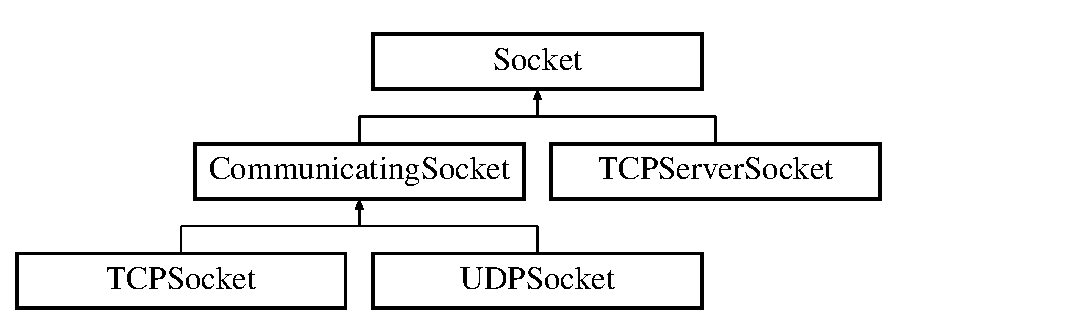
\includegraphics[height=3.000000cm]{classSocket}
\end{center}
\end{figure}
\subsection*{Öffentliche Methoden}
\begin{DoxyCompactItemize}
\item 
\hypertarget{classSocket_ad585c3f2a21f2511a5dea235923c59ee}{{\bfseries Socket} (unsigned short local\-Port)}\label{classSocket_ad585c3f2a21f2511a5dea235923c59ee}

\item 
\hypertarget{classSocket_a32ef908835f62b11ba5b86c18a0bfe28}{{\bfseries Socket} (unsigned short remote\-Addr, unsigned short remote\-Port)}\label{classSocket_a32ef908835f62b11ba5b86c18a0bfe28}

\item 
\hypertarget{classSocket_a2d8cf63685c29463181d8e5536e0f3cc}{void {\bfseries set\-Remote\-Addr} (unsigned short remote\-Addr)}\label{classSocket_a2d8cf63685c29463181d8e5536e0f3cc}

\item 
\hypertarget{classSocket_a54dd43a68403812d58ea9e2e8024cf45}{void {\bfseries set\-Remote\-Port} (unsigned short remote\-Port)}\label{classSocket_a54dd43a68403812d58ea9e2e8024cf45}

\item 
\hypertarget{classSocket_a773fe4a35146002de76952e16fdebcfa}{void {\bfseries set\-Local\-Port} (unsigned short local\-Port)}\label{classSocket_a773fe4a35146002de76952e16fdebcfa}

\item 
\hypertarget{classSocket_a2bcd6d8cca7a9dfd88b3101732d0abcc}{unsigned short {\bfseries get\-Socket\-Descriptor} ()}\label{classSocket_a2bcd6d8cca7a9dfd88b3101732d0abcc}

\item 
\hypertarget{classSocket_a5774a66b0f9d58380bf248c08c0dd33c}{unsigned int $\ast$ {\bfseries get\-Remote\-Addr} ()}\label{classSocket_a5774a66b0f9d58380bf248c08c0dd33c}

\item 
\hyperlink{classSocket_aeac4eb6379a543d38ed88977d3b6630a}{$\sim$\-Socket} ()
\item 
string \hyperlink{classSocket_a0fca07bdfa97874fba1a17995ed7cda3}{get\-Local\-Address} ()  throw (\-Socket\-Exception)
\item 
unsigned short \hyperlink{classSocket_ae01143b667d69483a2f53d0f4ce7eeed}{get\-Local\-Port} ()  throw (\-Socket\-Exception)
\item 
void \hyperlink{classSocket_a773fe4a35146002de76952e16fdebcfa}{set\-Local\-Port} (unsigned short local\-Port)  throw (\-Socket\-Exception)
\item 
void \hyperlink{classSocket_aa6b986410bc2e606ba27d01fa7cb8836}{set\-Local\-Address\-And\-Port} (const string \&local\-Address, unsigned short local\-Port=0)  throw (\-Socket\-Exception)
\end{DoxyCompactItemize}
\subsection*{Öffentliche, statische Methoden}
\begin{DoxyCompactItemize}
\item 
static void \hyperlink{classSocket_ac5060aeb501044044351d5a85b3fc95f}{clean\-Up} ()  throw (\-Socket\-Exception)
\item 
static unsigned short \hyperlink{classSocket_a982c63b25c5b756321a74074a275adbc}{resolve\-Service} (const string \&service, const string \&protocol=\char`\"{}tcp\char`\"{})
\end{DoxyCompactItemize}
\subsection*{Geschützte Methoden}
\begin{DoxyCompactItemize}
\item 
\hypertarget{classSocket_a53e00027bab2125a2b407914c6148589}{{\bfseries Socket} (int type, int protocol)  throw (\-Socket\-Exception)}\label{classSocket_a53e00027bab2125a2b407914c6148589}

\item 
\hypertarget{classSocket_a6a2609eef6559336a595a336f138d395}{{\bfseries Socket} (int sock\-Desc)}\label{classSocket_a6a2609eef6559336a595a336f138d395}

\end{DoxyCompactItemize}
\subsection*{Geschützte Attribute}
\begin{DoxyCompactItemize}
\item 
\hypertarget{classSocket_ad5704d2fdfb062139e1f88831617bbfb}{int {\bfseries sock\-Desc}}\label{classSocket_ad5704d2fdfb062139e1f88831617bbfb}

\end{DoxyCompactItemize}


\subsection{Ausführliche Beschreibung}
Base class representing basic communication endpoint 

\subsection{Beschreibung der Konstruktoren und Destruktoren}
\hypertarget{classSocket_aeac4eb6379a543d38ed88977d3b6630a}{\index{Socket@{Socket}!$\sim$\-Socket@{$\sim$\-Socket}}
\index{$\sim$\-Socket@{$\sim$\-Socket}!Socket@{Socket}}
\subsubsection[{$\sim$\-Socket}]{\setlength{\rightskip}{0pt plus 5cm}Socket\-::$\sim$\-Socket (
\begin{DoxyParamCaption}
{}
\end{DoxyParamCaption}
)}}\label{classSocket_aeac4eb6379a543d38ed88977d3b6630a}
Close and deallocate this socket 

\subsection{Dokumentation der Elementfunktionen}
\hypertarget{classSocket_ac5060aeb501044044351d5a85b3fc95f}{\index{Socket@{Socket}!clean\-Up@{clean\-Up}}
\index{clean\-Up@{clean\-Up}!Socket@{Socket}}
\subsubsection[{clean\-Up}]{\setlength{\rightskip}{0pt plus 5cm}void Socket\-::clean\-Up (
\begin{DoxyParamCaption}
{}
\end{DoxyParamCaption}
) throw  {\bf Socket\-Exception}) \hspace{0.3cm}{\ttfamily [static]}}}\label{classSocket_ac5060aeb501044044351d5a85b3fc95f}
If Win\-Sock, unload the Win\-Sock D\-L\-Ls; otherwise do nothing. We ignore this in our sample client code but include it in the library for completeness. If you are running on Windows and you are concerned about D\-L\-L resource consumption, call this after you are done with all \hyperlink{classSocket}{Socket} instances. If you execute this on Windows while some instance of \hyperlink{classSocket}{Socket} exists, you are toast. For portability of client code, this is an empty function on non-\/\-Windows platforms so you can always include it. 
\begin{DoxyParams}{Parameter}
{\em buffer} & buffer to receive the data \\
\hline
{\em buffer\-Len} & maximum number of bytes to read into buffer \\
\hline
\end{DoxyParams}
\begin{DoxyReturn}{Rückgabe}
number of bytes read, 0 for E\-O\-F, and -\/1 for error 
\end{DoxyReturn}

\begin{DoxyExceptions}{Ausnahmebehandlung}
{\em \hyperlink{classSocketException}{Socket\-Exception}} & thrown Win\-Sock clean up fails \\
\hline
\end{DoxyExceptions}
\hypertarget{classSocket_a0fca07bdfa97874fba1a17995ed7cda3}{\index{Socket@{Socket}!get\-Local\-Address@{get\-Local\-Address}}
\index{get\-Local\-Address@{get\-Local\-Address}!Socket@{Socket}}
\subsubsection[{get\-Local\-Address}]{\setlength{\rightskip}{0pt plus 5cm}string Socket\-::get\-Local\-Address (
\begin{DoxyParamCaption}
{}
\end{DoxyParamCaption}
) throw  {\bf Socket\-Exception}) }}\label{classSocket_a0fca07bdfa97874fba1a17995ed7cda3}
Get the local address \begin{DoxyReturn}{Rückgabe}
local address of socket 
\end{DoxyReturn}

\begin{DoxyExceptions}{Ausnahmebehandlung}
{\em \hyperlink{classSocketException}{Socket\-Exception}} & thrown if fetch fails \\
\hline
\end{DoxyExceptions}
\hypertarget{classSocket_ae01143b667d69483a2f53d0f4ce7eeed}{\index{Socket@{Socket}!get\-Local\-Port@{get\-Local\-Port}}
\index{get\-Local\-Port@{get\-Local\-Port}!Socket@{Socket}}
\subsubsection[{get\-Local\-Port}]{\setlength{\rightskip}{0pt plus 5cm}unsigned short Socket\-::get\-Local\-Port (
\begin{DoxyParamCaption}
{}
\end{DoxyParamCaption}
) throw  {\bf Socket\-Exception}) }}\label{classSocket_ae01143b667d69483a2f53d0f4ce7eeed}
Get the local port \begin{DoxyReturn}{Rückgabe}
local port of socket 
\end{DoxyReturn}

\begin{DoxyExceptions}{Ausnahmebehandlung}
{\em \hyperlink{classSocketException}{Socket\-Exception}} & thrown if fetch fails \\
\hline
\end{DoxyExceptions}
\hypertarget{classSocket_a982c63b25c5b756321a74074a275adbc}{\index{Socket@{Socket}!resolve\-Service@{resolve\-Service}}
\index{resolve\-Service@{resolve\-Service}!Socket@{Socket}}
\subsubsection[{resolve\-Service}]{\setlength{\rightskip}{0pt plus 5cm}unsigned short Socket\-::resolve\-Service (
\begin{DoxyParamCaption}
\item[{const string \&}]{service, }
\item[{const string \&}]{protocol = {\ttfamily \char`\"{}tcp\char`\"{}}}
\end{DoxyParamCaption}
)\hspace{0.3cm}{\ttfamily [static]}}}\label{classSocket_a982c63b25c5b756321a74074a275adbc}
Resolve the specified service for the specified protocol to the corresponding port number in host byte order 
\begin{DoxyParams}{Parameter}
{\em service} & service to resolve (e.\-g., \char`\"{}http\char`\"{}) \\
\hline
{\em protocol} & protocol of service to resolve. Default is \char`\"{}tcp\char`\"{}. \\
\hline
\end{DoxyParams}
\hypertarget{classSocket_aa6b986410bc2e606ba27d01fa7cb8836}{\index{Socket@{Socket}!set\-Local\-Address\-And\-Port@{set\-Local\-Address\-And\-Port}}
\index{set\-Local\-Address\-And\-Port@{set\-Local\-Address\-And\-Port}!Socket@{Socket}}
\subsubsection[{set\-Local\-Address\-And\-Port}]{\setlength{\rightskip}{0pt plus 5cm}void Socket\-::set\-Local\-Address\-And\-Port (
\begin{DoxyParamCaption}
\item[{const string \&}]{local\-Address, }
\item[{unsigned short}]{local\-Port = {\ttfamily 0}}
\end{DoxyParamCaption}
) throw  {\bf Socket\-Exception}) }}\label{classSocket_aa6b986410bc2e606ba27d01fa7cb8836}
Set the local port to the specified port and the local address to the specified address. If you omit the port, a random port will be selected. 
\begin{DoxyParams}{Parameter}
{\em local\-Address} & local address \\
\hline
{\em local\-Port} & local port \\
\hline
\end{DoxyParams}

\begin{DoxyExceptions}{Ausnahmebehandlung}
{\em \hyperlink{classSocketException}{Socket\-Exception}} & thrown if setting local port or address fails \\
\hline
\end{DoxyExceptions}
\hypertarget{classSocket_a773fe4a35146002de76952e16fdebcfa}{\index{Socket@{Socket}!set\-Local\-Port@{set\-Local\-Port}}
\index{set\-Local\-Port@{set\-Local\-Port}!Socket@{Socket}}
\subsubsection[{set\-Local\-Port}]{\setlength{\rightskip}{0pt plus 5cm}void Socket\-::set\-Local\-Port (
\begin{DoxyParamCaption}
\item[{unsigned short}]{local\-Port}
\end{DoxyParamCaption}
) throw  {\bf Socket\-Exception}) }}\label{classSocket_a773fe4a35146002de76952e16fdebcfa}
Set the local port to the specified port and the local address to any interface 
\begin{DoxyParams}{Parameter}
{\em local\-Port} & local port \\
\hline
\end{DoxyParams}

\begin{DoxyExceptions}{Ausnahmebehandlung}
{\em \hyperlink{classSocketException}{Socket\-Exception}} & thrown if setting local port fails \\
\hline
\end{DoxyExceptions}


Die Dokumentation für diese Klasse wurde erzeugt aufgrund der Dateien\-:\begin{DoxyCompactItemize}
\item 
Communication.\-h\item 
Practical\-Socket.\-h\item 
Communication.\-cpp\item 
Practical\-Socket.\-cpp\end{DoxyCompactItemize}

\hypertarget{classSocketException}{\section{Socket\-Exception Klassenreferenz}
\label{classSocketException}\index{Socket\-Exception@{Socket\-Exception}}
}


{\ttfamily \#include $<$Practical\-Socket.\-h$>$}

Klassendiagramm für Socket\-Exception\-:\begin{figure}[H]
\begin{center}
\leavevmode
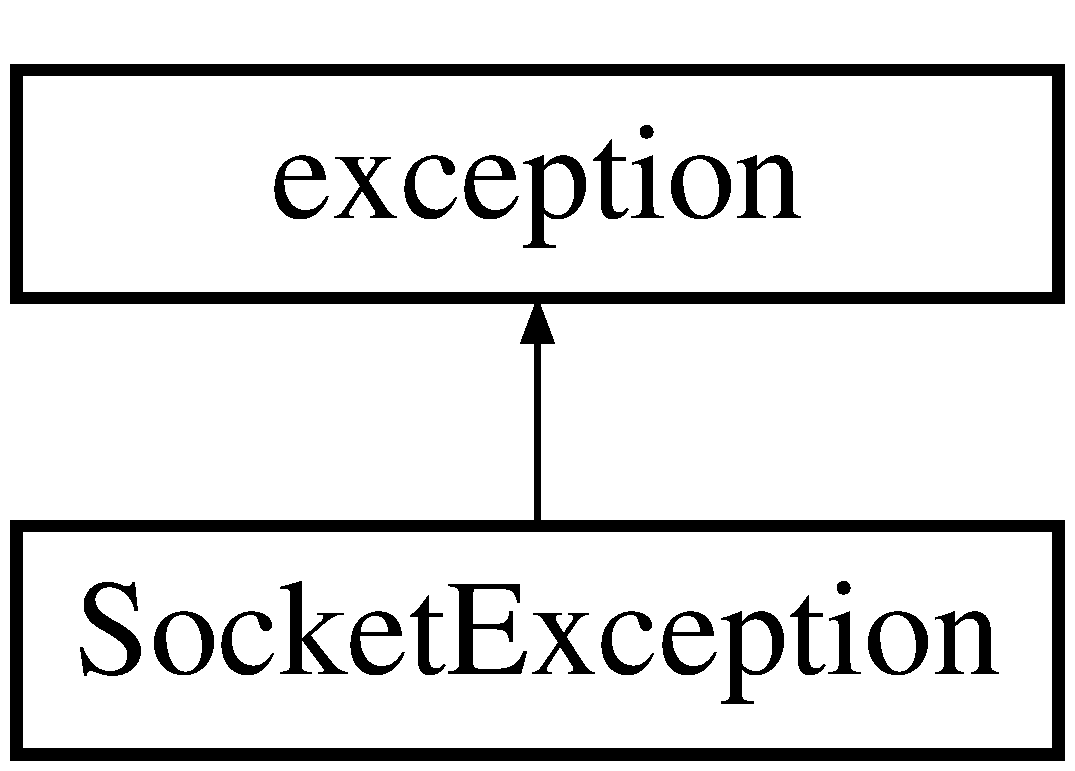
\includegraphics[height=2.000000cm]{classSocketException}
\end{center}
\end{figure}
\subsection*{Öffentliche Methoden}
\begin{DoxyCompactItemize}
\item 
\hyperlink{classSocketException_abb5bcecd9d9e20868c237ec5a82cf5c3}{Socket\-Exception} (const string \&message, bool incl\-Sys\-Msg=false)  throw ()
\item 
\hyperlink{classSocketException_a659557c899329aea01977c980c4db9b9}{$\sim$\-Socket\-Exception} ()  throw ()
\item 
const char $\ast$ \hyperlink{classSocketException_a06b7b3f186976bb5ec7e7bf007c4f0ac}{what} () const   throw ()
\end{DoxyCompactItemize}


\subsection{Ausführliche Beschreibung}
Zeigt ein Problem mit der Ausf"uhrung eines Socketaufrufs an. 

\subsection{Beschreibung der Konstruktoren und Destruktoren}
\hypertarget{classSocketException_abb5bcecd9d9e20868c237ec5a82cf5c3}{\index{Socket\-Exception@{Socket\-Exception}!Socket\-Exception@{Socket\-Exception}}
\index{Socket\-Exception@{Socket\-Exception}!SocketException@{Socket\-Exception}}
\subsubsection[{Socket\-Exception}]{\setlength{\rightskip}{0pt plus 5cm}Socket\-Exception\-::\-Socket\-Exception (
\begin{DoxyParamCaption}
\item[{const string \&}]{message, }
\item[{bool}]{incl\-Sys\-Msg = {\ttfamily false}}
\end{DoxyParamCaption}
) throw  ) }}\label{classSocketException_abb5bcecd9d9e20868c237ec5a82cf5c3}
Erzeugt eine \char`\"{}\-Socket\-Exception\char`\"{} mit einem erkl"arenden Hinweistext. 
\begin{DoxyParams}{Parameter}
{\em message} & Nachricht die den Fehlern beschreibt \\
\hline
{\em inc\-Sys\-Msg} & true falls eine Systemnachricht (von strerror(errno)) sollte zu der f"ur den User bereitgestellten Nachricht hinzugef"ugt werden. \\
\hline
\end{DoxyParams}
\hypertarget{classSocketException_a659557c899329aea01977c980c4db9b9}{\index{Socket\-Exception@{Socket\-Exception}!$\sim$\-Socket\-Exception@{$\sim$\-Socket\-Exception}}
\index{$\sim$\-Socket\-Exception@{$\sim$\-Socket\-Exception}!SocketException@{Socket\-Exception}}
\subsubsection[{$\sim$\-Socket\-Exception}]{\setlength{\rightskip}{0pt plus 5cm}Socket\-Exception\-::$\sim$\-Socket\-Exception (
\begin{DoxyParamCaption}
{}
\end{DoxyParamCaption}
) throw  ) }}\label{classSocketException_a659557c899329aea01977c980c4db9b9}
Nur bereitgestellt um zu gew"ahrleisten, dass keine Exceptions zur"uckgeworfen / zur"uckgegeben werden. 

\subsection{Dokumentation der Elementfunktionen}
\hypertarget{classSocketException_a06b7b3f186976bb5ec7e7bf007c4f0ac}{\index{Socket\-Exception@{Socket\-Exception}!what@{what}}
\index{what@{what}!SocketException@{Socket\-Exception}}
\subsubsection[{what}]{\setlength{\rightskip}{0pt plus 5cm}const char $\ast$ Socket\-Exception\-::what (
\begin{DoxyParamCaption}
{}
\end{DoxyParamCaption}
) const throw  ) }}\label{classSocketException_a06b7b3f186976bb5ec7e7bf007c4f0ac}
Holt die Exception-\/\-Nachricht. \begin{DoxyReturn}{Rückgabe}
Exception-\/\-Nachricht. 
\end{DoxyReturn}


Die Dokumentation für diese Klasse wurde erzeugt aufgrund der Dateien\-:\begin{DoxyCompactItemize}
\item 
Practical\-Socket.\-h\item 
Practical\-Socket.\-cpp\end{DoxyCompactItemize}

\hypertarget{structT__nuex}{\section{T\-\_\-nuex Struct Reference}
\label{structT__nuex}\index{T\-\_\-nuex@{T\-\_\-nuex}}
}
\subsection*{Public Attributes}
\begin{DoxyCompactItemize}
\item 
\hypertarget{structT__nuex_a9b27fdca5f3fb081e5880a1e5c258638}{short int {\bfseries testen} \mbox{[}401\mbox{]}}\label{structT__nuex_a9b27fdca5f3fb081e5880a1e5c258638}

\end{DoxyCompactItemize}


The documentation for this struct was generated from the following file\-:\begin{DoxyCompactItemize}
\item 
mab.\-cpp\end{DoxyCompactItemize}

\hypertarget{classTCPServerSocket}{\section{T\-C\-P\-Server\-Socket Klassenreferenz}
\label{classTCPServerSocket}\index{T\-C\-P\-Server\-Socket@{T\-C\-P\-Server\-Socket}}
}


{\ttfamily \#include $<$Practical\-Socket.\-h$>$}

Klassendiagramm für T\-C\-P\-Server\-Socket\-:\begin{figure}[H]
\begin{center}
\leavevmode
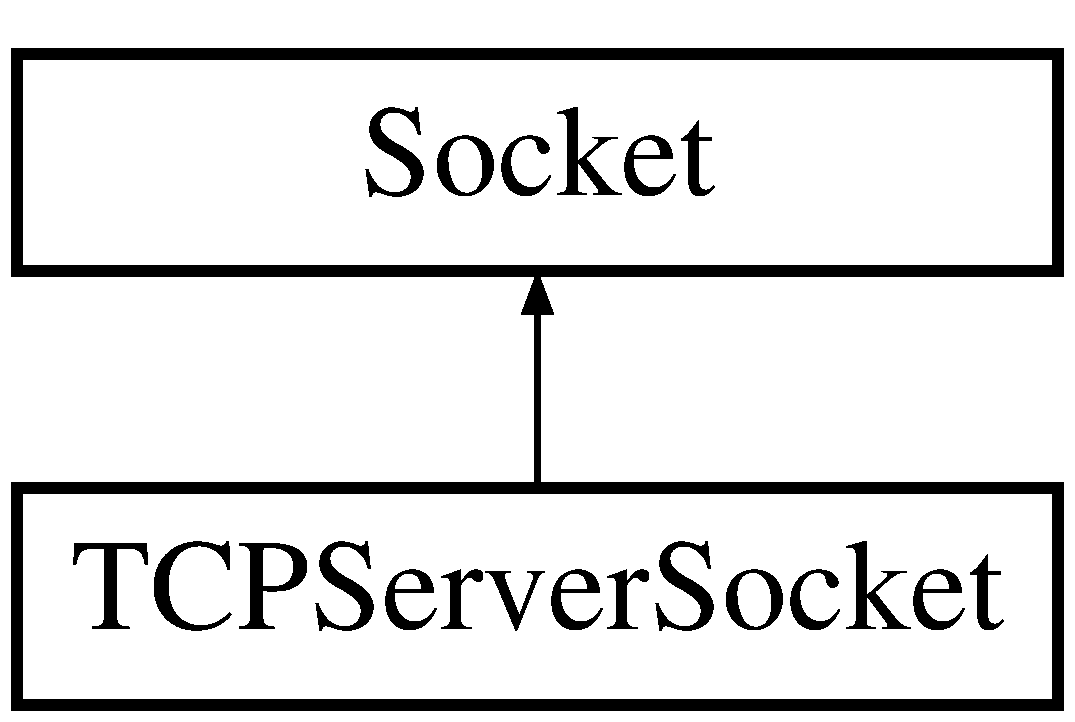
\includegraphics[height=2.000000cm]{classTCPServerSocket}
\end{center}
\end{figure}
\subsection*{Öffentliche Methoden}
\begin{DoxyCompactItemize}
\item 
\hyperlink{classTCPServerSocket_ae559a3154527d09fe14a8e5ee1f53d7a}{T\-C\-P\-Server\-Socket} (unsigned short local\-Port, int queue\-Len=5)  throw (\-Socket\-Exception)
\item 
\hyperlink{classTCPServerSocket_a3908fecb1b038f7c14fcc7726f54d01d}{T\-C\-P\-Server\-Socket} (const string \&local\-Address, unsigned short local\-Port, int queue\-Len=5)  throw (\-Socket\-Exception)
\item 
\hyperlink{classTCPSocket}{T\-C\-P\-Socket} $\ast$ \hyperlink{classTCPServerSocket_a1d161137e1b069de7a7bfc14d3f8212c}{accept} ()  throw (\-Socket\-Exception)
\end{DoxyCompactItemize}
\subsection*{Weitere Geerbte Elemente}


\subsection{Ausführliche Beschreibung}
T\-C\-P-\/\-Socket Klasse f"ur Server. 

\subsection{Beschreibung der Konstruktoren und Destruktoren}
\hypertarget{classTCPServerSocket_ae559a3154527d09fe14a8e5ee1f53d7a}{\index{T\-C\-P\-Server\-Socket@{T\-C\-P\-Server\-Socket}!T\-C\-P\-Server\-Socket@{T\-C\-P\-Server\-Socket}}
\index{T\-C\-P\-Server\-Socket@{T\-C\-P\-Server\-Socket}!TCPServerSocket@{T\-C\-P\-Server\-Socket}}
\subsubsection[{T\-C\-P\-Server\-Socket}]{\setlength{\rightskip}{0pt plus 5cm}T\-C\-P\-Server\-Socket\-::\-T\-C\-P\-Server\-Socket (
\begin{DoxyParamCaption}
\item[{unsigned short}]{local\-Port, }
\item[{int}]{queue\-Len = {\ttfamily 5}}
\end{DoxyParamCaption}
) throw  {\bf Socket\-Exception}) }}\label{classTCPServerSocket_ae559a3154527d09fe14a8e5ee1f53d7a}
Erzeugt einen T\-C\-P-\/\-Socket f"ur die Nutzung mit dem Server, welcher zu einer beliebigen Schnittstelle auf dem vereinbarten Port Verbindungen zul"asst. 
\begin{DoxyParams}{Parameter}
{\em local\-Port} & Lokaler Port des Server. \\
\hline
{\em queue\-Len} & Maximale Warteschlangenl"ange f"ur ausstehende Verbindungsanfragen. (default 5) \\
\hline
\end{DoxyParams}

\begin{DoxyExceptions}{Ausnahmebehandlung}
{\em \hyperlink{classSocketException}{Socket\-Exception}} & wird geworfen falls es nicht m"oglich ist einen \hyperlink{classSocket}{Socket} zu erzeugen. \\
\hline
\end{DoxyExceptions}
\hypertarget{classTCPServerSocket_a3908fecb1b038f7c14fcc7726f54d01d}{\index{T\-C\-P\-Server\-Socket@{T\-C\-P\-Server\-Socket}!T\-C\-P\-Server\-Socket@{T\-C\-P\-Server\-Socket}}
\index{T\-C\-P\-Server\-Socket@{T\-C\-P\-Server\-Socket}!TCPServerSocket@{T\-C\-P\-Server\-Socket}}
\subsubsection[{T\-C\-P\-Server\-Socket}]{\setlength{\rightskip}{0pt plus 5cm}T\-C\-P\-Server\-Socket\-::\-T\-C\-P\-Server\-Socket (
\begin{DoxyParamCaption}
\item[{const string \&}]{local\-Address, }
\item[{unsigned short}]{local\-Port, }
\item[{int}]{queue\-Len = {\ttfamily 5}}
\end{DoxyParamCaption}
) throw  {\bf Socket\-Exception}) }}\label{classTCPServerSocket_a3908fecb1b038f7c14fcc7726f54d01d}
Erzeugt einen T\-C\-P-\/\-Socket f"ur die Nutzung mit dem Server, welcher zu einer beliebigen Schnittstelle zu einer vereinbarten Adresse Verbindungen zul"asst. 
\begin{DoxyParams}{Parameter}
{\em local\-Address} & Lokales Interface (Adresse) des Server-\/\-Sockets. \\
\hline
{\em local\-Port} & Lokaler Port des Servers. \\
\hline
{\em queue\-Len} & Maximale Warteschlangenl"ange f"ur ausstehende Verbindungsanfragen. (default 5) \\
\hline
\end{DoxyParams}

\begin{DoxyExceptions}{Ausnahmebehandlung}
{\em \hyperlink{classSocketException}{Socket\-Exception}} & wird geworfen, falls es nicht m"oglich ist einen \hyperlink{classSocket}{Socket} zu erzeugen. \\
\hline
\end{DoxyExceptions}


\subsection{Dokumentation der Elementfunktionen}
\hypertarget{classTCPServerSocket_a1d161137e1b069de7a7bfc14d3f8212c}{\index{T\-C\-P\-Server\-Socket@{T\-C\-P\-Server\-Socket}!accept@{accept}}
\index{accept@{accept}!TCPServerSocket@{T\-C\-P\-Server\-Socket}}
\subsubsection[{accept}]{\setlength{\rightskip}{0pt plus 5cm}{\bf T\-C\-P\-Socket} $\ast$ T\-C\-P\-Server\-Socket\-::accept (
\begin{DoxyParamCaption}
{}
\end{DoxyParamCaption}
) throw  {\bf Socket\-Exception}) }}\label{classTCPServerSocket_a1d161137e1b069de7a7bfc14d3f8212c}
Blockiert solange bis eine neue Verbindung auf diesem \hyperlink{classSocket}{Socket} etabliert wurde oder ein Fehler auftritt. \begin{DoxyReturn}{Rückgabe}
Neue Socketverbindung 
\end{DoxyReturn}

\begin{DoxyExceptions}{Ausnahmebehandlung}
{\em \hyperlink{classSocketException}{Socket\-Exception}} & wird geworfen falls der Versuch eine neue Verbindung zu erzeugen fehlschl"agt. \\
\hline
\end{DoxyExceptions}


Die Dokumentation für diese Klasse wurde erzeugt aufgrund der Dateien\-:\begin{DoxyCompactItemize}
\item 
Practical\-Socket.\-h\item 
Practical\-Socket.\-cpp\end{DoxyCompactItemize}

\hypertarget{classTCPSocket}{\section{T\-C\-P\-Socket Klassenreferenz}
\label{classTCPSocket}\index{T\-C\-P\-Socket@{T\-C\-P\-Socket}}
}


{\ttfamily \#include $<$Practical\-Socket.\-h$>$}

Klassendiagramm für T\-C\-P\-Socket\-:\begin{figure}[H]
\begin{center}
\leavevmode
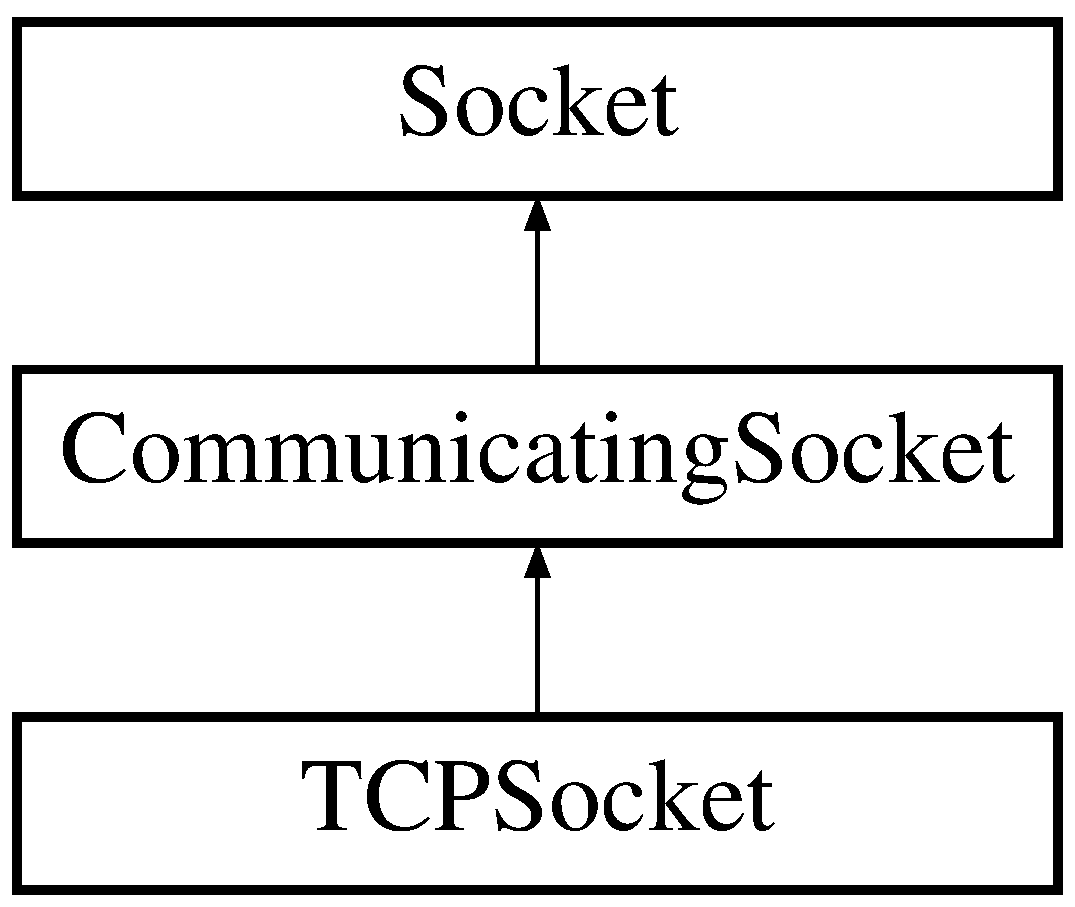
\includegraphics[height=3.000000cm]{classTCPSocket}
\end{center}
\end{figure}
\subsection*{Öffentliche Methoden}
\begin{DoxyCompactItemize}
\item 
\hyperlink{classTCPSocket_a7a50427a401d1a6f3209d51818bad901}{T\-C\-P\-Socket} ()  throw (\-Socket\-Exception)
\item 
\hyperlink{classTCPSocket_a7b246b66f6dc3246ab2777b771e5f917}{T\-C\-P\-Socket} (const string \&foreign\-Address, unsigned short foreign\-Port)  throw (\-Socket\-Exception)
\end{DoxyCompactItemize}
\subsection*{Freundbeziehungen}
\begin{DoxyCompactItemize}
\item 
\hypertarget{classTCPSocket_ae8bcdc0d25881a17b23e557296236fa9}{class {\bfseries T\-C\-P\-Server\-Socket}}\label{classTCPSocket_ae8bcdc0d25881a17b23e557296236fa9}

\end{DoxyCompactItemize}
\subsection*{Weitere Geerbte Elemente}


\subsection{Ausführliche Beschreibung}
T\-C\-P socket for communication with other T\-C\-P sockets 

\subsection{Beschreibung der Konstruktoren und Destruktoren}
\hypertarget{classTCPSocket_a7a50427a401d1a6f3209d51818bad901}{\index{T\-C\-P\-Socket@{T\-C\-P\-Socket}!T\-C\-P\-Socket@{T\-C\-P\-Socket}}
\index{T\-C\-P\-Socket@{T\-C\-P\-Socket}!TCPSocket@{T\-C\-P\-Socket}}
\subsubsection[{T\-C\-P\-Socket}]{\setlength{\rightskip}{0pt plus 5cm}T\-C\-P\-Socket\-::\-T\-C\-P\-Socket (
\begin{DoxyParamCaption}
{}
\end{DoxyParamCaption}
) throw  {\bf Socket\-Exception}) }}\label{classTCPSocket_a7a50427a401d1a6f3209d51818bad901}
Construct a T\-C\-P socket with no connection 
\begin{DoxyExceptions}{Ausnahmebehandlung}
{\em \hyperlink{classSocketException}{Socket\-Exception}} & thrown if unable to create T\-C\-P socket \\
\hline
\end{DoxyExceptions}
\hypertarget{classTCPSocket_a7b246b66f6dc3246ab2777b771e5f917}{\index{T\-C\-P\-Socket@{T\-C\-P\-Socket}!T\-C\-P\-Socket@{T\-C\-P\-Socket}}
\index{T\-C\-P\-Socket@{T\-C\-P\-Socket}!TCPSocket@{T\-C\-P\-Socket}}
\subsubsection[{T\-C\-P\-Socket}]{\setlength{\rightskip}{0pt plus 5cm}T\-C\-P\-Socket\-::\-T\-C\-P\-Socket (
\begin{DoxyParamCaption}
\item[{const string \&}]{foreign\-Address, }
\item[{unsigned short}]{foreign\-Port}
\end{DoxyParamCaption}
) throw  {\bf Socket\-Exception}) }}\label{classTCPSocket_a7b246b66f6dc3246ab2777b771e5f917}
Construct a T\-C\-P socket with a connection to the given foreign address and port 
\begin{DoxyParams}{Parameter}
{\em foreign\-Address} & foreign address (I\-P address or name) \\
\hline
{\em foreign\-Port} & foreign port \\
\hline
\end{DoxyParams}

\begin{DoxyExceptions}{Ausnahmebehandlung}
{\em \hyperlink{classSocketException}{Socket\-Exception}} & thrown if unable to create T\-C\-P socket \\
\hline
\end{DoxyExceptions}


Die Dokumentation für diese Klasse wurde erzeugt aufgrund der Dateien\-:\begin{DoxyCompactItemize}
\item 
Practical\-Socket.\-h\item 
Practical\-Socket.\-cpp\end{DoxyCompactItemize}

\hypertarget{classUDPSocket}{\section{U\-D\-P\-Socket Klassenreferenz}
\label{classUDPSocket}\index{U\-D\-P\-Socket@{U\-D\-P\-Socket}}
}


{\ttfamily \#include $<$Practical\-Socket.\-h$>$}

Klassendiagramm für U\-D\-P\-Socket\-:\begin{figure}[H]
\begin{center}
\leavevmode
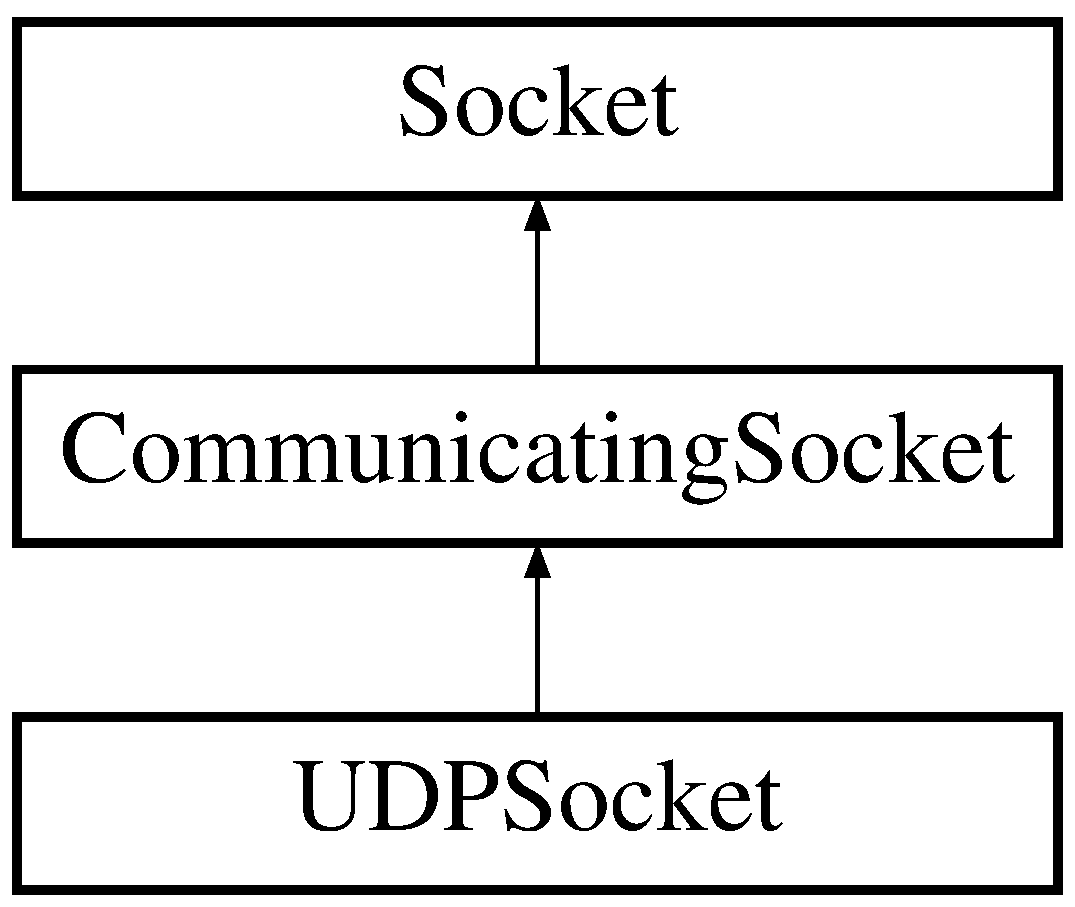
\includegraphics[height=3.000000cm]{classUDPSocket}
\end{center}
\end{figure}
\subsection*{Öffentliche Methoden}
\begin{DoxyCompactItemize}
\item 
\hyperlink{classUDPSocket_a4f86f3023f5a08f6355802599a10e100}{U\-D\-P\-Socket} ()  throw (\-Socket\-Exception)
\item 
\hyperlink{classUDPSocket_a14dcb55c4b60b12d4a7fff648cbb825f}{U\-D\-P\-Socket} (unsigned short local\-Port)  throw (\-Socket\-Exception)
\item 
\hyperlink{classUDPSocket_af19281c523f15ed30d7d78f09033713d}{U\-D\-P\-Socket} (const string \&local\-Address, unsigned short local\-Port)  throw (\-Socket\-Exception)
\item 
void \hyperlink{classUDPSocket_a7482e8e61cef160e1a7c0d6ac15c01be}{disconnect} ()  throw (\-Socket\-Exception)
\item 
void \hyperlink{classUDPSocket_a41a3595e226f273953cbd38618af5d5b}{send\-To} (const void $\ast$buffer, int buffer\-Len, const string \&foreign\-Address, unsigned short foreign\-Port)  throw (\-Socket\-Exception)
\item 
int \hyperlink{classUDPSocket_abcd5c064e2496bd8b1888fd4e1b68949}{recv\-From} (void $\ast$buffer, int buffer\-Len, string \&source\-Address, unsigned short \&source\-Port)  throw (\-Socket\-Exception)
\item 
void \hyperlink{classUDPSocket_a4dcfff33b45d1b84b5a602fc6f4a27f8}{set\-Multicast\-T\-T\-L} (unsigned char multicast\-T\-T\-L)  throw (\-Socket\-Exception)
\item 
void \hyperlink{classUDPSocket_a1b20c1e8bd49a9bd9b53dd4f1c8d4c11}{join\-Group} (const string \&multicast\-Group)  throw (\-Socket\-Exception)
\item 
void \hyperlink{classUDPSocket_a78835eaeca8a5ac039b4579c795e3640}{leave\-Group} (const string \&multicast\-Group)  throw (\-Socket\-Exception)
\end{DoxyCompactItemize}
\subsection*{Weitere Geerbte Elemente}


\subsection{Ausführliche Beschreibung}
U\-D\-P-\/\-Socket Klasse 

\subsection{Beschreibung der Konstruktoren und Destruktoren}
\hypertarget{classUDPSocket_a4f86f3023f5a08f6355802599a10e100}{\index{U\-D\-P\-Socket@{U\-D\-P\-Socket}!U\-D\-P\-Socket@{U\-D\-P\-Socket}}
\index{U\-D\-P\-Socket@{U\-D\-P\-Socket}!UDPSocket@{U\-D\-P\-Socket}}
\subsubsection[{U\-D\-P\-Socket}]{\setlength{\rightskip}{0pt plus 5cm}U\-D\-P\-Socket\-::\-U\-D\-P\-Socket (
\begin{DoxyParamCaption}
{}
\end{DoxyParamCaption}
) throw  {\bf Socket\-Exception}) }}\label{classUDPSocket_a4f86f3023f5a08f6355802599a10e100}
Erzeugt einen U\-D\-P-\/\-Socket. 
\begin{DoxyExceptions}{Ausnahmebehandlung}
{\em \hyperlink{classSocketException}{Socket\-Exception}} & wird geworfen falls die Erzeugung fehlschl"agt. \\
\hline
\end{DoxyExceptions}
\hypertarget{classUDPSocket_a14dcb55c4b60b12d4a7fff648cbb825f}{\index{U\-D\-P\-Socket@{U\-D\-P\-Socket}!U\-D\-P\-Socket@{U\-D\-P\-Socket}}
\index{U\-D\-P\-Socket@{U\-D\-P\-Socket}!UDPSocket@{U\-D\-P\-Socket}}
\subsubsection[{U\-D\-P\-Socket}]{\setlength{\rightskip}{0pt plus 5cm}U\-D\-P\-Socket\-::\-U\-D\-P\-Socket (
\begin{DoxyParamCaption}
\item[{unsigned short}]{local\-Port}
\end{DoxyParamCaption}
) throw  {\bf Socket\-Exception}) }}\label{classUDPSocket_a14dcb55c4b60b12d4a7fff648cbb825f}
Erzeugt einen U\-D\-P-\/\-Socket mit einem spezifischen Port. 
\begin{DoxyParams}{Parameter}
{\em local\-Port} & Lokaler Port \\
\hline
\end{DoxyParams}

\begin{DoxyExceptions}{Ausnahmebehandlung}
{\em \hyperlink{classSocketException}{Socket\-Exception}} & wird geworfen falls die Erzeugung fehlschl"agt. \\
\hline
\end{DoxyExceptions}
\hypertarget{classUDPSocket_af19281c523f15ed30d7d78f09033713d}{\index{U\-D\-P\-Socket@{U\-D\-P\-Socket}!U\-D\-P\-Socket@{U\-D\-P\-Socket}}
\index{U\-D\-P\-Socket@{U\-D\-P\-Socket}!UDPSocket@{U\-D\-P\-Socket}}
\subsubsection[{U\-D\-P\-Socket}]{\setlength{\rightskip}{0pt plus 5cm}U\-D\-P\-Socket\-::\-U\-D\-P\-Socket (
\begin{DoxyParamCaption}
\item[{const string \&}]{local\-Address, }
\item[{unsigned short}]{local\-Port}
\end{DoxyParamCaption}
) throw  {\bf Socket\-Exception}) }}\label{classUDPSocket_af19281c523f15ed30d7d78f09033713d}
Erzeugt einen U\-D\-P-\/\-Socket mit einer spezifischen Adresse und einem gegebenen Port. 
\begin{DoxyParams}{Parameter}
{\em local\-Address} & Lokale Adresse. \\
\hline
{\em local\-Port} & Lokaler Port. \\
\hline
\end{DoxyParams}

\begin{DoxyExceptions}{Ausnahmebehandlung}
{\em \hyperlink{classSocketException}{Socket\-Exception}} & wird geworfen falls die Erzeugung fehlschl"agt. \\
\hline
\end{DoxyExceptions}


\subsection{Dokumentation der Elementfunktionen}
\hypertarget{classUDPSocket_a7482e8e61cef160e1a7c0d6ac15c01be}{\index{U\-D\-P\-Socket@{U\-D\-P\-Socket}!disconnect@{disconnect}}
\index{disconnect@{disconnect}!UDPSocket@{U\-D\-P\-Socket}}
\subsubsection[{disconnect}]{\setlength{\rightskip}{0pt plus 5cm}void U\-D\-P\-Socket\-::disconnect (
\begin{DoxyParamCaption}
{}
\end{DoxyParamCaption}
) throw  {\bf Socket\-Exception}) }}\label{classUDPSocket_a7482e8e61cef160e1a7c0d6ac15c01be}
Setze Adresse und Port zur"uck. \begin{DoxyReturn}{Rückgabe}
true falls kein Fehler auftrat. 
\end{DoxyReturn}

\begin{DoxyExceptions}{Ausnahmebehandlung}
{\em \hyperlink{classSocketException}{Socket\-Exception}} & wird geworfen falls eine Trennung fehlschl"agt. \\
\hline
\end{DoxyExceptions}
\hypertarget{classUDPSocket_a1b20c1e8bd49a9bd9b53dd4f1c8d4c11}{\index{U\-D\-P\-Socket@{U\-D\-P\-Socket}!join\-Group@{join\-Group}}
\index{join\-Group@{join\-Group}!UDPSocket@{U\-D\-P\-Socket}}
\subsubsection[{join\-Group}]{\setlength{\rightskip}{0pt plus 5cm}void U\-D\-P\-Socket\-::join\-Group (
\begin{DoxyParamCaption}
\item[{const string \&}]{multicast\-Group}
\end{DoxyParamCaption}
) throw  {\bf Socket\-Exception}) }}\label{classUDPSocket_a1b20c1e8bd49a9bd9b53dd4f1c8d4c11}
Tritt der angegebenen Multicast-\/\-Gruppe bei. 
\begin{DoxyParams}{Parameter}
{\em multicast\-Group} & Adresse der Mutlicast-\/\-Gruppe. \\
\hline
\end{DoxyParams}

\begin{DoxyExceptions}{Ausnahmebehandlung}
{\em \hyperlink{classSocketException}{Socket\-Exception}} & wird geworfen falls das Beitreten fehlschl"agt. \\
\hline
\end{DoxyExceptions}
\hypertarget{classUDPSocket_a78835eaeca8a5ac039b4579c795e3640}{\index{U\-D\-P\-Socket@{U\-D\-P\-Socket}!leave\-Group@{leave\-Group}}
\index{leave\-Group@{leave\-Group}!UDPSocket@{U\-D\-P\-Socket}}
\subsubsection[{leave\-Group}]{\setlength{\rightskip}{0pt plus 5cm}void U\-D\-P\-Socket\-::leave\-Group (
\begin{DoxyParamCaption}
\item[{const string \&}]{multicast\-Group}
\end{DoxyParamCaption}
) throw  {\bf Socket\-Exception}) }}\label{classUDPSocket_a78835eaeca8a5ac039b4579c795e3640}
Verlasse die angegebene Multicast-\/\-Gruppe. 
\begin{DoxyParams}{Parameter}
{\em multicast\-Group} & Zu verlassende Multicast-\/\-Gruppe. \\
\hline
\end{DoxyParams}

\begin{DoxyExceptions}{Ausnahmebehandlung}
{\em \hyperlink{classSocketException}{Socket\-Exception}} & wird geworfen falls das Verlassen fehlschl"agt. \\
\hline
\end{DoxyExceptions}
\hypertarget{classUDPSocket_abcd5c064e2496bd8b1888fd4e1b68949}{\index{U\-D\-P\-Socket@{U\-D\-P\-Socket}!recv\-From@{recv\-From}}
\index{recv\-From@{recv\-From}!UDPSocket@{U\-D\-P\-Socket}}
\subsubsection[{recv\-From}]{\setlength{\rightskip}{0pt plus 5cm}int U\-D\-P\-Socket\-::recv\-From (
\begin{DoxyParamCaption}
\item[{void $\ast$}]{buffer, }
\item[{int}]{buffer\-Len, }
\item[{string \&}]{source\-Address, }
\item[{unsigned short \&}]{source\-Port}
\end{DoxyParamCaption}
) throw  {\bf Socket\-Exception}) }}\label{classUDPSocket_abcd5c064e2496bd8b1888fd4e1b68949}
Empf"angt eine Nachricht an einem U\-D\-P-\/\-Socket. 
\begin{DoxyParams}{Parameter}
{\em buffer} & Buffer in den gelesen werden soll. \\
\hline
{\em buffer\-Len} & Maximale Anzahl an Bytes die empfangen werden sollen. \\
\hline
{\em source\-Address} & Adresse von der die Nachricht stammt. \\
\hline
{\em source\-Port} & Portnummer des Senders. \\
\hline
\end{DoxyParams}
\begin{DoxyReturn}{Rückgabe}
Anzahl der Bytes die empfangen wurden, -\/1 falls ein Fehler auftrat. 
\end{DoxyReturn}

\begin{DoxyExceptions}{Ausnahmebehandlung}
{\em \hyperlink{classSocketException}{Socket\-Exception}} & wird geworfen falls das Empfangen fehlschl"agt. \\
\hline
\end{DoxyExceptions}
\hypertarget{classUDPSocket_a41a3595e226f273953cbd38618af5d5b}{\index{U\-D\-P\-Socket@{U\-D\-P\-Socket}!send\-To@{send\-To}}
\index{send\-To@{send\-To}!UDPSocket@{U\-D\-P\-Socket}}
\subsubsection[{send\-To}]{\setlength{\rightskip}{0pt plus 5cm}void U\-D\-P\-Socket\-::send\-To (
\begin{DoxyParamCaption}
\item[{const void $\ast$}]{buffer, }
\item[{int}]{buffer\-Len, }
\item[{const string \&}]{foreign\-Address, }
\item[{unsigned short}]{foreign\-Port}
\end{DoxyParamCaption}
) throw  {\bf Socket\-Exception}) }}\label{classUDPSocket_a41a3595e226f273953cbd38618af5d5b}
Sendet einen Buffer als U\-D\-P-\/\-Datagramm an eine bestimmte Adresse und Portnummer. 
\begin{DoxyParams}{Parameter}
{\em buffer} & Buffer der gesendet werden soll. \\
\hline
{\em buffer\-Len} & Anzahl der Bytes die geschrieben werden sollen. \\
\hline
{\em foreign\-Address} & Adresse an die versendet werden soll. \\
\hline
{\em foreign\-Port} & Portnummer an die versendet werden soll. \\
\hline
\end{DoxyParams}
\begin{DoxyReturn}{Rückgabe}
true falls Versandt geklappt hat. 
\end{DoxyReturn}

\begin{DoxyExceptions}{Ausnahmebehandlung}
{\em \hyperlink{classSocketException}{Socket\-Exception}} & wird geworfen falls das Senden fehlschl"agt. \\
\hline
\end{DoxyExceptions}
\hypertarget{classUDPSocket_a4dcfff33b45d1b84b5a602fc6f4a27f8}{\index{U\-D\-P\-Socket@{U\-D\-P\-Socket}!set\-Multicast\-T\-T\-L@{set\-Multicast\-T\-T\-L}}
\index{set\-Multicast\-T\-T\-L@{set\-Multicast\-T\-T\-L}!UDPSocket@{U\-D\-P\-Socket}}
\subsubsection[{set\-Multicast\-T\-T\-L}]{\setlength{\rightskip}{0pt plus 5cm}void U\-D\-P\-Socket\-::set\-Multicast\-T\-T\-L (
\begin{DoxyParamCaption}
\item[{unsigned char}]{multicast\-T\-T\-L}
\end{DoxyParamCaption}
) throw  {\bf Socket\-Exception}) }}\label{classUDPSocket_a4dcfff33b45d1b84b5a602fc6f4a27f8}
Setzt Multicast T\-T\-L. 
\begin{DoxyParams}{Parameter}
{\em multicast\-T\-T\-L} & Multicast T\-T\-L. \\
\hline
\end{DoxyParams}

\begin{DoxyExceptions}{Ausnahmebehandlung}
{\em \hyperlink{classSocketException}{Socket\-Exception}} & wird geworfen falls das Setzen fehlschl"agt. \\
\hline
\end{DoxyExceptions}


Die Dokumentation für diese Klasse wurde erzeugt aufgrund der Dateien\-:\begin{DoxyCompactItemize}
\item 
Practical\-Socket.\-h\item 
Practical\-Socket.\-cpp\end{DoxyCompactItemize}

%--- End generated contents ---

% Index
\newpage
\phantomsection
\addcontentsline{toc}{part}{Index}
\printindex

\end{document}
